\documentclass[twoside]{book}

% Packages required by doxygen
\usepackage{fixltx2e}
\usepackage{calc}
\usepackage{doxygen}
\usepackage{graphicx}
\usepackage[utf8]{inputenc}
\usepackage{makeidx}
\usepackage{multicol}
\usepackage{multirow}
\PassOptionsToPackage{warn}{textcomp}
\usepackage{textcomp}
\usepackage[nointegrals]{wasysym}
\usepackage[table]{xcolor}

% Font selection
\usepackage[T1]{fontenc}
\usepackage{mathptmx}
\usepackage[scaled=.90]{helvet}
\usepackage{courier}
\usepackage{amssymb}
\usepackage{sectsty}
\renewcommand{\familydefault}{\sfdefault}
\allsectionsfont{%
  \fontseries{bc}\selectfont%
  \color{darkgray}%
}
\renewcommand{\DoxyLabelFont}{%
  \fontseries{bc}\selectfont%
  \color{darkgray}%
}
\newcommand{\+}{\discretionary{\mbox{\scriptsize$\hookleftarrow$}}{}{}}

% Page & text layout
\usepackage{geometry}
\geometry{%
  a4paper,%
  top=2.5cm,%
  bottom=2.5cm,%
  left=2.5cm,%
  right=2.5cm%
}
\tolerance=750
\hfuzz=15pt
\hbadness=750
\setlength{\emergencystretch}{15pt}
\setlength{\parindent}{0cm}
\setlength{\parskip}{0.2cm}
\makeatletter
\renewcommand{\paragraph}{%
  \@startsection{paragraph}{4}{0ex}{-1.0ex}{1.0ex}{%
    \normalfont\normalsize\bfseries\SS@parafont%
  }%
}
\renewcommand{\subparagraph}{%
  \@startsection{subparagraph}{5}{0ex}{-1.0ex}{1.0ex}{%
    \normalfont\normalsize\bfseries\SS@subparafont%
  }%
}
\makeatother

% Headers & footers
\usepackage{fancyhdr}
\pagestyle{fancyplain}
\fancyhead[LE]{\fancyplain{}{\bfseries\thepage}}
\fancyhead[CE]{\fancyplain{}{}}
\fancyhead[RE]{\fancyplain{}{\bfseries\leftmark}}
\fancyhead[LO]{\fancyplain{}{\bfseries\rightmark}}
\fancyhead[CO]{\fancyplain{}{}}
\fancyhead[RO]{\fancyplain{}{\bfseries\thepage}}
\fancyfoot[LE]{\fancyplain{}{}}
\fancyfoot[CE]{\fancyplain{}{}}
\fancyfoot[RE]{\fancyplain{}{\bfseries\scriptsize Generated on Tue Jan 20 2015 17\+:12\+:52 for mitgcm by Doxygen }}
\fancyfoot[LO]{\fancyplain{}{\bfseries\scriptsize Generated on Tue Jan 20 2015 17\+:12\+:52 for mitgcm by Doxygen }}
\fancyfoot[CO]{\fancyplain{}{}}
\fancyfoot[RO]{\fancyplain{}{}}
\renewcommand{\footrulewidth}{0.4pt}
\renewcommand{\chaptermark}[1]{%
  \markboth{#1}{}%
}
\renewcommand{\sectionmark}[1]{%
  \markright{\thesection\ #1}%
}

% Indices & bibliography
\usepackage{natbib}
\usepackage[titles]{tocloft}
\setcounter{tocdepth}{3}
\setcounter{secnumdepth}{5}
\makeindex

% Hyperlinks (required, but should be loaded last)
\usepackage{ifpdf}
\ifpdf
  \usepackage[pdftex,pagebackref=true]{hyperref}
\else
  \usepackage[ps2pdf,pagebackref=true]{hyperref}
\fi
\hypersetup{%
  colorlinks=true,%
  linkcolor=blue,%
  citecolor=blue,%
  unicode%
}

% Custom commands
\newcommand{\clearemptydoublepage}{%
  \newpage{\pagestyle{empty}\cleardoublepage}%
}


%===== C O N T E N T S =====

\begin{document}

% Titlepage & ToC
\hypersetup{pageanchor=false,
             bookmarks=true,
             bookmarksnumbered=true,
             pdfencoding=unicode
            }
\pagenumbering{roman}
\begin{titlepage}
\vspace*{7cm}
\begin{center}%
{\Large mitgcm }\\
\vspace*{1cm}
{\large Generated by Doxygen 1.8.8}\\
\vspace*{0.5cm}
{\small Tue Jan 20 2015 17:12:52}\\
\end{center}
\end{titlepage}
\clearemptydoublepage
\tableofcontents
\clearemptydoublepage
\pagenumbering{arabic}
\hypersetup{pageanchor=true}

%--- Begin generated contents ---
\chapter{Documentation for python package mitgcm}
\label{index}\hypertarget{index}{}\begin{DoxyAuthor}{Author}
Ed Doddridge
\end{DoxyAuthor}
\hypertarget{index_Overview}{}\section{Overview}\label{index_Overview}
This package provides methods and classes for analysing the output of mitgcm simulations.\hypertarget{index_Revision}{}\section{History}\label{index_Revision}
January 2015\+: Added documentation

February 2015\+: Added streamline and streakline algorithms 
\chapter{Hierarchical Index}
\section{Class Hierarchy}
This inheritance list is sorted roughly, but not completely, alphabetically\+:\begin{DoxyCompactList}
\item dict\begin{DoxyCompactList}
\item \contentsline{section}{mitgcm.\+core.\+M\+I\+Tgcm\+\_\+\+Simulation}{\pageref{classmitgcm_1_1core_1_1MITgcm__Simulation}}{}
\begin{DoxyCompactList}
\item \contentsline{section}{mitgcm.\+core.\+Grid}{\pageref{classmitgcm_1_1core_1_1Grid}}{}
\item \contentsline{section}{mitgcm.\+core.\+Tracerpoint\+\_\+field}{\pageref{classmitgcm_1_1core_1_1Tracerpoint__field}}{}
\begin{DoxyCompactList}
\item \contentsline{section}{mitgcm.\+core.\+Bernoulli}{\pageref{classmitgcm_1_1core_1_1Bernoulli}}{}
\item \contentsline{section}{mitgcm.\+core.\+Density}{\pageref{classmitgcm_1_1core_1_1Density}}{}
\item \contentsline{section}{mitgcm.\+core.\+Free\+\_\+surface}{\pageref{classmitgcm_1_1core_1_1Free__surface}}{}
\item \contentsline{section}{mitgcm.\+core.\+Potential\+\_\+vorticity}{\pageref{classmitgcm_1_1core_1_1Potential__vorticity}}{}
\item \contentsline{section}{mitgcm.\+core.\+Pressure}{\pageref{classmitgcm_1_1core_1_1Pressure}}{}
\item \contentsline{section}{mitgcm.\+core.\+Temperature}{\pageref{classmitgcm_1_1core_1_1Temperature}}{}
\end{DoxyCompactList}
\item \contentsline{section}{mitgcm.\+core.\+Upoint\+\_\+field}{\pageref{classmitgcm_1_1core_1_1Upoint__field}}{}
\item \contentsline{section}{mitgcm.\+core.\+Vorticitypoint\+\_\+field}{\pageref{classmitgcm_1_1core_1_1Vorticitypoint__field}}{}
\begin{DoxyCompactList}
\item \contentsline{section}{mitgcm.\+core.\+Vorticity}{\pageref{classmitgcm_1_1core_1_1Vorticity}}{}
\end{DoxyCompactList}
\item \contentsline{section}{mitgcm.\+core.\+Vpoint\+\_\+field}{\pageref{classmitgcm_1_1core_1_1Vpoint__field}}{}
\item \contentsline{section}{mitgcm.\+core.\+Wpoint\+\_\+field}{\pageref{classmitgcm_1_1core_1_1Wpoint__field}}{}
\end{DoxyCompactList}
\end{DoxyCompactList}
\end{DoxyCompactList}

\chapter{Class Index}
\section{Class List}
Here are the classes, structs, unions and interfaces with brief descriptions\+:\begin{DoxyCompactList}
\item\contentsline{section}{\hyperlink{classmitgcm_1_1core_1_1Bernoulli}{mitgcm.\+core.\+Bernoulli} \\*The \hyperlink{classmitgcm_1_1core_1_1Bernoulli}{Bernoulli} field, evaluated from velocity, pressure and density }{\pageref{classmitgcm_1_1core_1_1Bernoulli}}{}
\item\contentsline{section}{\hyperlink{classmitgcm_1_1core_1_1Density}{mitgcm.\+core.\+Density} }{\pageref{classmitgcm_1_1core_1_1Density}}{}
\item\contentsline{section}{\hyperlink{classmitgcm_1_1core_1_1Free__surface}{mitgcm.\+core.\+Free\+\_\+surface} }{\pageref{classmitgcm_1_1core_1_1Free__surface}}{}
\item\contentsline{section}{\hyperlink{classmitgcm_1_1core_1_1Grid}{mitgcm.\+core.\+Grid} \\*This defines the class for the grid object }{\pageref{classmitgcm_1_1core_1_1Grid}}{}
\item\contentsline{section}{\hyperlink{classmitgcm_1_1core_1_1MITgcm__Simulation}{mitgcm.\+core.\+M\+I\+Tgcm\+\_\+\+Simulation} \\*The simulation class is the main class of this package, and an instance of this class is a model object }{\pageref{classmitgcm_1_1core_1_1MITgcm__Simulation}}{}
\item\contentsline{section}{\hyperlink{classmitgcm_1_1core_1_1Potential__vorticity}{mitgcm.\+core.\+Potential\+\_\+vorticity} \\*Evaluate the potential vorticity on the tracer points }{\pageref{classmitgcm_1_1core_1_1Potential__vorticity}}{}
\item\contentsline{section}{\hyperlink{classmitgcm_1_1core_1_1Pressure}{mitgcm.\+core.\+Pressure} }{\pageref{classmitgcm_1_1core_1_1Pressure}}{}
\item\contentsline{section}{\hyperlink{classmitgcm_1_1core_1_1Temperature}{mitgcm.\+core.\+Temperature} }{\pageref{classmitgcm_1_1core_1_1Temperature}}{}
\item\contentsline{section}{\hyperlink{classmitgcm_1_1core_1_1Tracerpoint__field}{mitgcm.\+core.\+Tracerpoint\+\_\+field} \\*This is the base class for all model fields on the tracer points }{\pageref{classmitgcm_1_1core_1_1Tracerpoint__field}}{}
\item\contentsline{section}{\hyperlink{classmitgcm_1_1core_1_1Upoint__field}{mitgcm.\+core.\+Upoint\+\_\+field} \\*This is the class for all fields on zonal velocity points }{\pageref{classmitgcm_1_1core_1_1Upoint__field}}{}
\item\contentsline{section}{\hyperlink{classmitgcm_1_1core_1_1Vorticity}{mitgcm.\+core.\+Vorticity} }{\pageref{classmitgcm_1_1core_1_1Vorticity}}{}
\item\contentsline{section}{\hyperlink{classmitgcm_1_1core_1_1Vorticitypoint__field}{mitgcm.\+core.\+Vorticitypoint\+\_\+field} }{\pageref{classmitgcm_1_1core_1_1Vorticitypoint__field}}{}
\item\contentsline{section}{\hyperlink{classmitgcm_1_1core_1_1Vpoint__field}{mitgcm.\+core.\+Vpoint\+\_\+field} \\*This is the class for all fields on meridional velocity points }{\pageref{classmitgcm_1_1core_1_1Vpoint__field}}{}
\item\contentsline{section}{\hyperlink{classmitgcm_1_1core_1_1Wpoint__field}{mitgcm.\+core.\+Wpoint\+\_\+field} \\*This is the class for all fields on vertical velocity points }{\pageref{classmitgcm_1_1core_1_1Wpoint__field}}{}
\end{DoxyCompactList}

\chapter{Class Documentation}
\hypertarget{classmitgcm_1_1Bernoulli}{\section{mitgcm.\+Bernoulli Class Reference}
\label{classmitgcm_1_1Bernoulli}\index{mitgcm.\+Bernoulli@{mitgcm.\+Bernoulli}}
}


The \hyperlink{classmitgcm_1_1Bernoulli}{Bernoulli} field, evaluated from velocity, pressure and density.  


Inheritance diagram for mitgcm.\+Bernoulli\+:\begin{figure}[H]
\begin{center}
\leavevmode
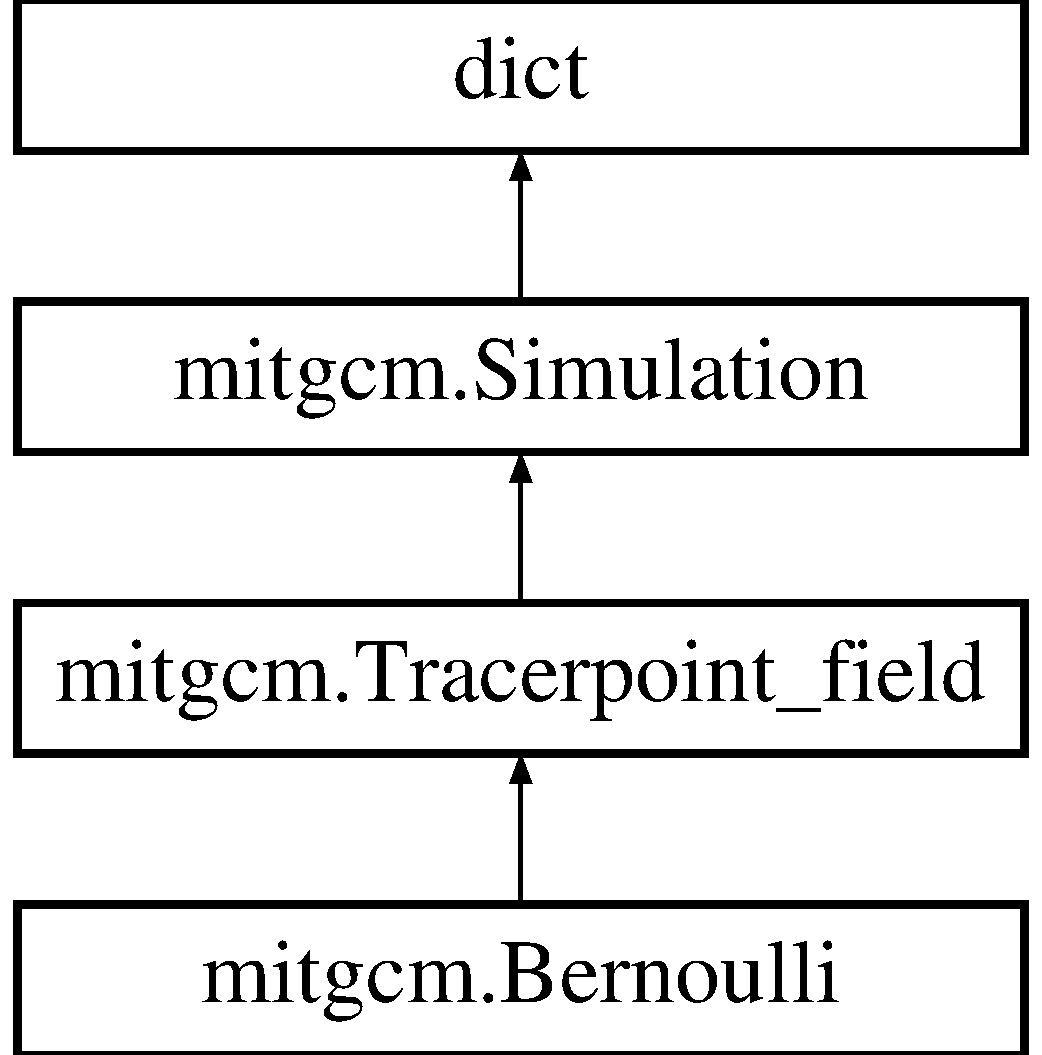
\includegraphics[height=4.000000cm]{classmitgcm_1_1Bernoulli}
\end{center}
\end{figure}
\subsection*{Public Member Functions}
\begin{DoxyCompactItemize}
\item 
\hypertarget{classmitgcm_1_1Bernoulli_a5f78ab27df77454ef131f5c24ca8dbf9}{def {\bfseries \+\_\+\+\_\+init\+\_\+\+\_\+}}\label{classmitgcm_1_1Bernoulli_a5f78ab27df77454ef131f5c24ca8dbf9}

\end{DoxyCompactItemize}
\subsection*{Additional Inherited Members}


\subsection{Detailed Description}
The \hyperlink{classmitgcm_1_1Bernoulli}{Bernoulli} field, evaluated from velocity, pressure and density. 



Definition at line 667 of file \+\_\+\+\_\+init\+\_\+\+\_\+.\+py.



The documentation for this class was generated from the following file\+:\begin{DoxyCompactItemize}
\item 
\+\_\+\+\_\+init\+\_\+\+\_\+.\+py\end{DoxyCompactItemize}

\hypertarget{classmitgcm_1_1Density}{\section{mitgcm.\+Density Class Reference}
\label{classmitgcm_1_1Density}\index{mitgcm.\+Density@{mitgcm.\+Density}}
}
Inheritance diagram for mitgcm.\+Density\+:\begin{figure}[H]
\begin{center}
\leavevmode
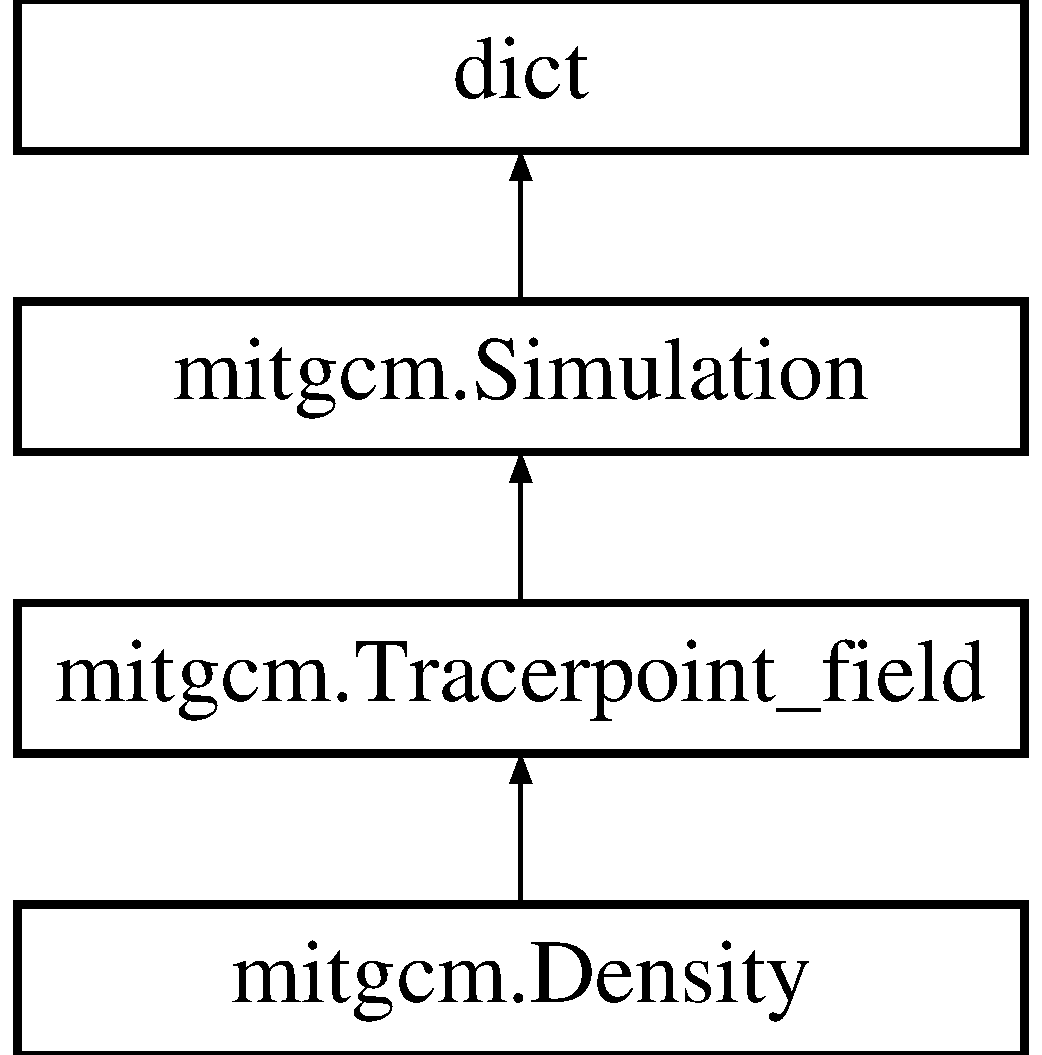
\includegraphics[height=4.000000cm]{classmitgcm_1_1Density}
\end{center}
\end{figure}
\subsection*{Public Member Functions}
\begin{DoxyCompactItemize}
\item 
\hypertarget{classmitgcm_1_1Density_aebdb54f40c181a305136c8d877c188d1}{def {\bfseries \+\_\+\+\_\+init\+\_\+\+\_\+}}\label{classmitgcm_1_1Density_aebdb54f40c181a305136c8d877c188d1}

\item 
\hypertarget{classmitgcm_1_1Density_a8838db86600856226b8856ae1b0ab7e6}{def {\bfseries calculate\+\_\+\+Tot\+Rho\+Tend}}\label{classmitgcm_1_1Density_a8838db86600856226b8856ae1b0ab7e6}

\end{DoxyCompactItemize}
\subsection*{Additional Inherited Members}


\subsection{Detailed Description}


Definition at line 640 of file \+\_\+\+\_\+init\+\_\+\+\_\+.\+py.



The documentation for this class was generated from the following file\+:\begin{DoxyCompactItemize}
\item 
\+\_\+\+\_\+init\+\_\+\+\_\+.\+py\end{DoxyCompactItemize}

\hypertarget{classmitgcm_1_1Free__surface}{\section{mitgcm.\+Free\+\_\+surface Class Reference}
\label{classmitgcm_1_1Free__surface}\index{mitgcm.\+Free\+\_\+surface@{mitgcm.\+Free\+\_\+surface}}
}
Inheritance diagram for mitgcm.\+Free\+\_\+surface\+:\begin{figure}[H]
\begin{center}
\leavevmode
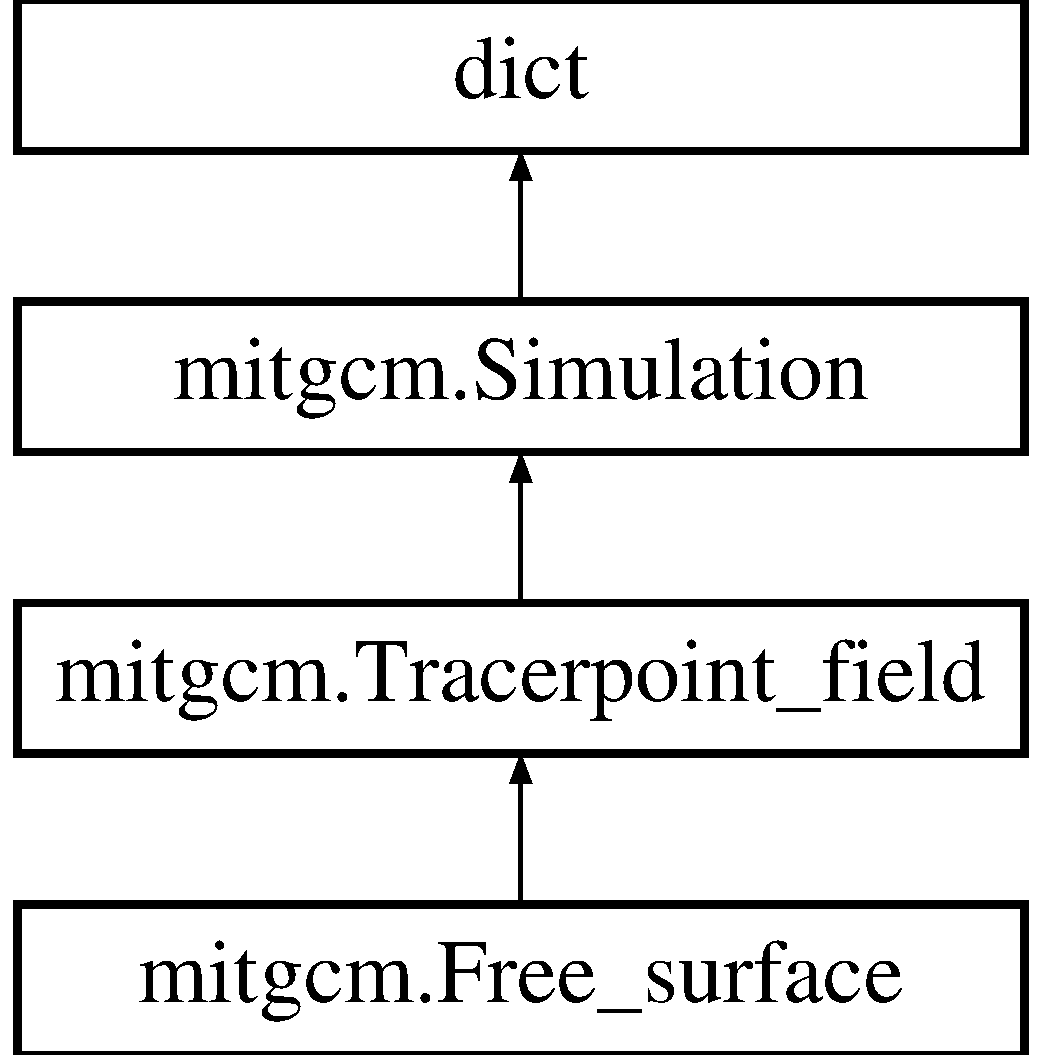
\includegraphics[height=4.000000cm]{classmitgcm_1_1Free__surface}
\end{center}
\end{figure}
\subsection*{Public Member Functions}
\begin{DoxyCompactItemize}
\item 
\hypertarget{classmitgcm_1_1Free__surface_a92630a9966a8f863bfa7d58aa844ad41}{def {\bfseries \+\_\+\+\_\+init\+\_\+\+\_\+}}\label{classmitgcm_1_1Free__surface_a92630a9966a8f863bfa7d58aa844ad41}

\end{DoxyCompactItemize}
\subsection*{Additional Inherited Members}


\subsection{Detailed Description}


Definition at line 667 of file \+\_\+\+\_\+init\+\_\+\+\_\+.\+py.



The documentation for this class was generated from the following file\+:\begin{DoxyCompactItemize}
\item 
\+\_\+\+\_\+init\+\_\+\+\_\+.\+py\end{DoxyCompactItemize}

\hypertarget{classmitgcm_1_1Grid}{\section{mitgcm.\+Grid Class Reference}
\label{classmitgcm_1_1Grid}\index{mitgcm.\+Grid@{mitgcm.\+Grid}}
}


This defines the class for the grid object.  


Inheritance diagram for mitgcm.\+Grid\+:\begin{figure}[H]
\begin{center}
\leavevmode
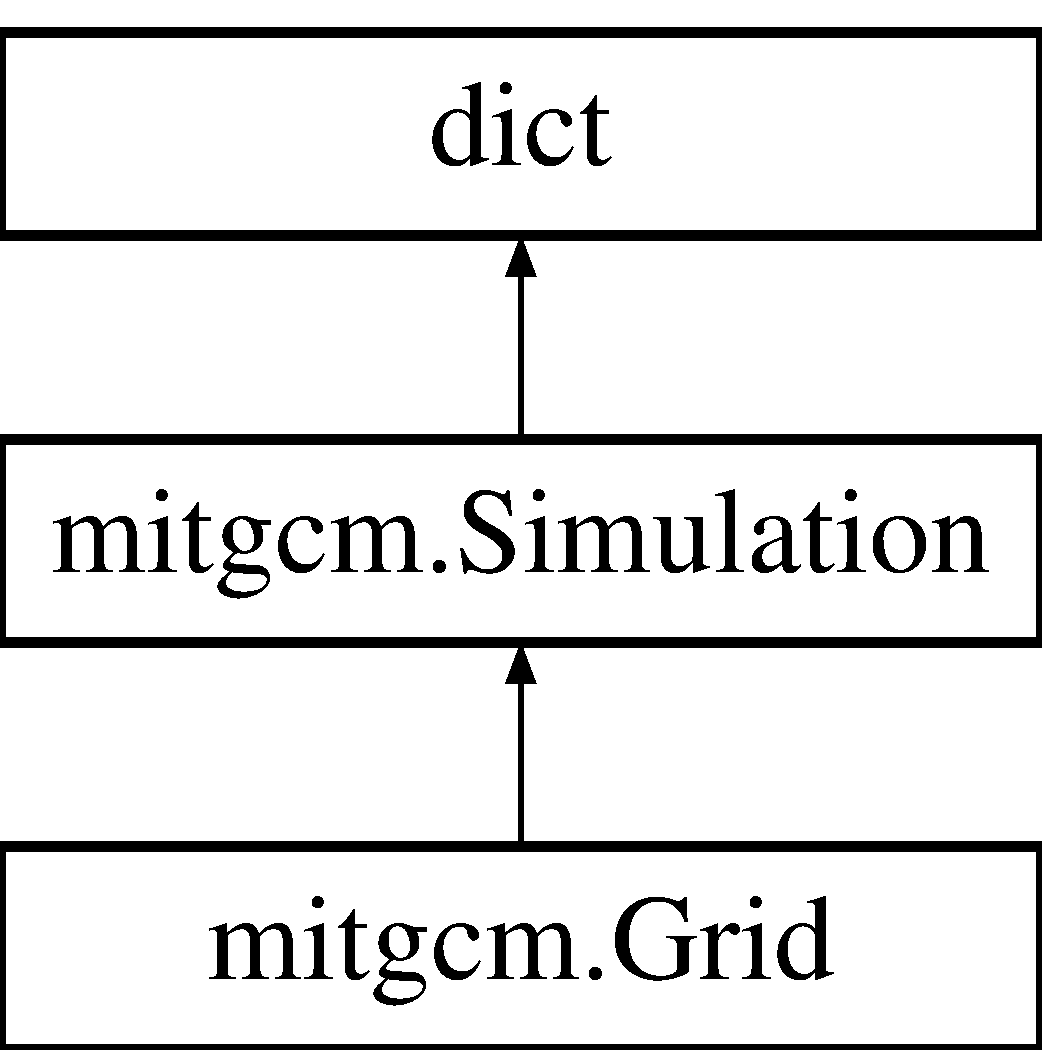
\includegraphics[height=3.000000cm]{classmitgcm_1_1Grid}
\end{center}
\end{figure}
\subsection*{Public Member Functions}
\begin{DoxyCompactItemize}
\item 
def \hyperlink{classmitgcm_1_1Grid_a156118c888f3135853c7c3c493c03232}{\+\_\+\+\_\+init\+\_\+\+\_\+}
\begin{DoxyCompactList}\small\item\em Define a single object that has all of the grid variables tucked away in it. \end{DoxyCompactList}\end{DoxyCompactItemize}
\subsection*{Static Public Attributes}
\begin{DoxyCompactItemize}
\item 
\hypertarget{classmitgcm_1_1Grid_aa45aab99b16e38406392f0be871fb6b4}{tuple {\bfseries grid\+\_\+netcdf\+\_\+file} = net\+C\+D\+F4.\+Dataset(grid\+\_\+netcdf\+\_\+filename)}\label{classmitgcm_1_1Grid_aa45aab99b16e38406392f0be871fb6b4}

\end{DoxyCompactItemize}
\subsection*{Additional Inherited Members}


\subsection{Detailed Description}
This defines the class for the grid object. 

This object holds all the information about the grid on which the simulation was run. It also holds mask for getting only the boundary values of fields on the tracer points. \begin{DoxyVerb}This class is the only one that isn't written to use dicts - this should be fixed at some stage. \end{DoxyVerb}
 

Definition at line 543 of file \+\_\+\+\_\+init\+\_\+\+\_\+.\+py.



\subsection{Constructor \& Destructor Documentation}
\hypertarget{classmitgcm_1_1Grid_a156118c888f3135853c7c3c493c03232}{\index{mitgcm\+::\+Grid@{mitgcm\+::\+Grid}!\+\_\+\+\_\+init\+\_\+\+\_\+@{\+\_\+\+\_\+init\+\_\+\+\_\+}}
\index{\+\_\+\+\_\+init\+\_\+\+\_\+@{\+\_\+\+\_\+init\+\_\+\+\_\+}!mitgcm\+::\+Grid@{mitgcm\+::\+Grid}}
\subsubsection[{\+\_\+\+\_\+init\+\_\+\+\_\+}]{\setlength{\rightskip}{0pt plus 5cm}def mitgcm.\+Grid.\+\_\+\+\_\+init\+\_\+\+\_\+ (
\begin{DoxyParamCaption}
\item[{}]{self, }
\item[{}]{grid\+\_\+netcdf\+\_\+filename}
\end{DoxyParamCaption}
)}}\label{classmitgcm_1_1Grid_a156118c888f3135853c7c3c493c03232}


Define a single object that has all of the grid variables tucked away in it. 

Each of the variables pulled directly from the netcdf file still has the original description attached to it. The 2\+D and 3\+D arrays do not. 

Definition at line 549 of file \+\_\+\+\_\+init\+\_\+\+\_\+.\+py.



The documentation for this class was generated from the following file\+:\begin{DoxyCompactItemize}
\item 
\+\_\+\+\_\+init\+\_\+\+\_\+.\+py\end{DoxyCompactItemize}

\hypertarget{classmitgcm_1_1Potential__vorticity}{\section{mitgcm.\+Potential\+\_\+vorticity Class Reference}
\label{classmitgcm_1_1Potential__vorticity}\index{mitgcm.\+Potential\+\_\+vorticity@{mitgcm.\+Potential\+\_\+vorticity}}
}


Evaluate the potential vorticity on the tracer points.  


Inheritance diagram for mitgcm.\+Potential\+\_\+vorticity\+:\begin{figure}[H]
\begin{center}
\leavevmode
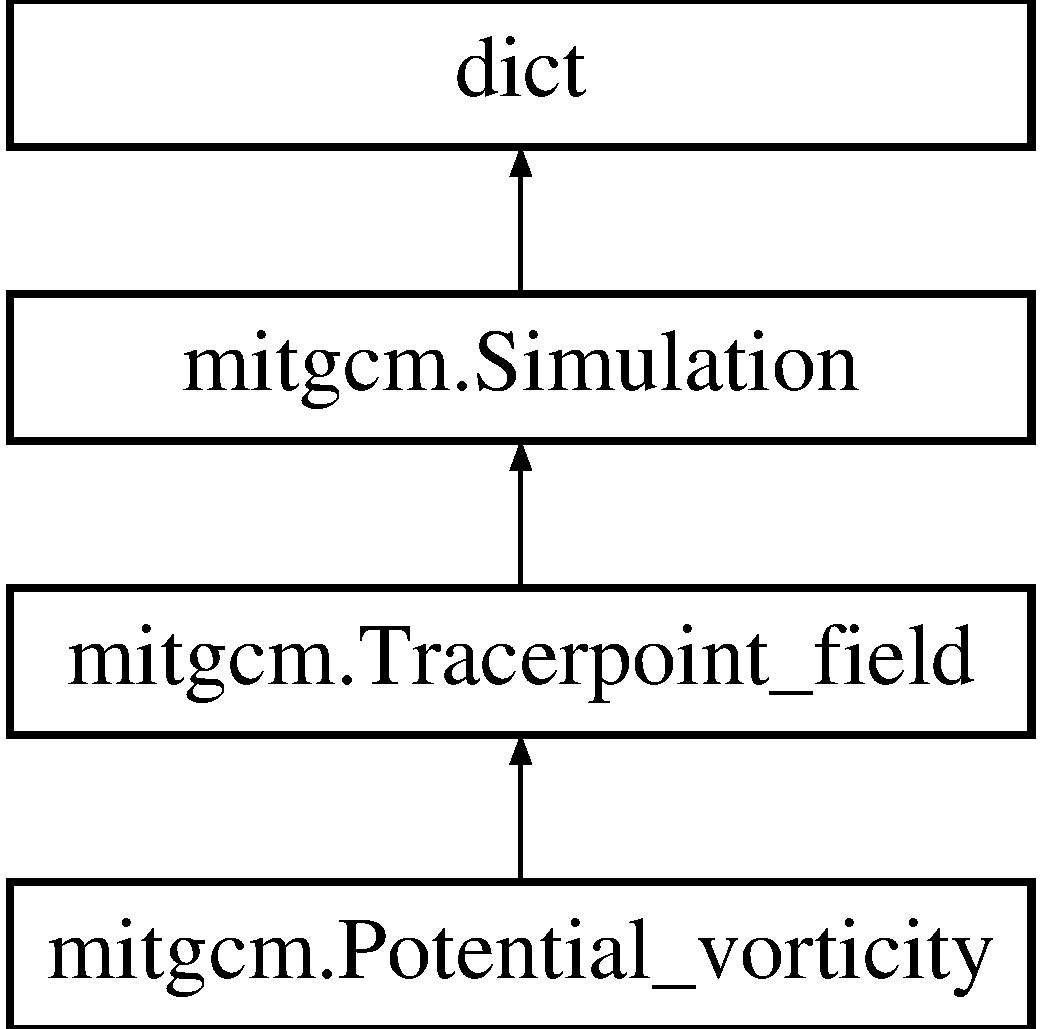
\includegraphics[height=4.000000cm]{classmitgcm_1_1Potential__vorticity}
\end{center}
\end{figure}
\subsection*{Public Member Functions}
\begin{DoxyCompactItemize}
\item 
\hypertarget{classmitgcm_1_1Potential__vorticity_a5412ecfe6e02d7a6953cf8c2a7dab4cb}{def {\bfseries \+\_\+\+\_\+init\+\_\+\+\_\+}}\label{classmitgcm_1_1Potential__vorticity_a5412ecfe6e02d7a6953cf8c2a7dab4cb}

\end{DoxyCompactItemize}
\subsection*{Additional Inherited Members}


\subsection{Detailed Description}
Evaluate the potential vorticity on the tracer points. 



Definition at line 718 of file \+\_\+\+\_\+init\+\_\+\+\_\+.\+py.



The documentation for this class was generated from the following file\+:\begin{DoxyCompactItemize}
\item 
\+\_\+\+\_\+init\+\_\+\+\_\+.\+py\end{DoxyCompactItemize}

\hypertarget{classmitgcm_1_1Pressure}{\section{mitgcm.\+Pressure Class Reference}
\label{classmitgcm_1_1Pressure}\index{mitgcm.\+Pressure@{mitgcm.\+Pressure}}
}
Inheritance diagram for mitgcm.\+Pressure\+:\begin{figure}[H]
\begin{center}
\leavevmode
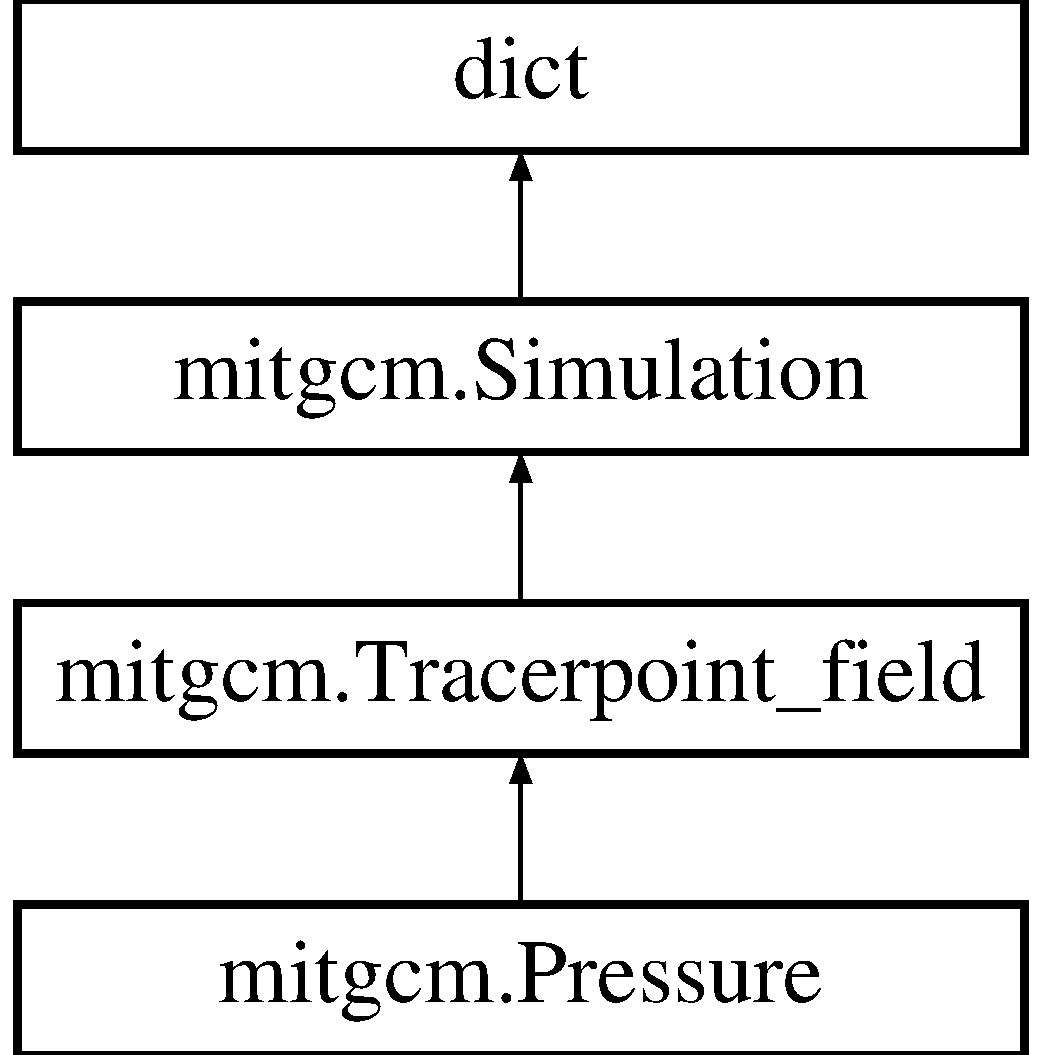
\includegraphics[height=4.000000cm]{classmitgcm_1_1Pressure}
\end{center}
\end{figure}
\subsection*{Public Member Functions}
\begin{DoxyCompactItemize}
\item 
\hypertarget{classmitgcm_1_1Pressure_a8233e6b8676c7405e760cdfea4f1bde3}{def {\bfseries \+\_\+\+\_\+init\+\_\+\+\_\+}}\label{classmitgcm_1_1Pressure_a8233e6b8676c7405e760cdfea4f1bde3}

\end{DoxyCompactItemize}
\subsection*{Additional Inherited Members}


\subsection{Detailed Description}


Definition at line 689 of file \+\_\+\+\_\+init\+\_\+\+\_\+.\+py.



The documentation for this class was generated from the following file\+:\begin{DoxyCompactItemize}
\item 
\+\_\+\+\_\+init\+\_\+\+\_\+.\+py\end{DoxyCompactItemize}

\hypertarget{classmitgcm_1_1Simulation}{\section{mitgcm.\+Simulation Class Reference}
\label{classmitgcm_1_1Simulation}\index{mitgcm.\+Simulation@{mitgcm.\+Simulation}}
}


The simulation class is the main class of this package, and an instance of this class is a model object.  


Inheritance diagram for mitgcm.\+Simulation\+:\begin{figure}[H]
\begin{center}
\leavevmode
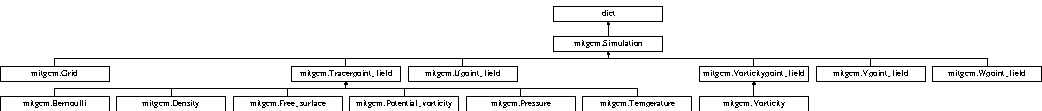
\includegraphics[height=1.490353cm]{classmitgcm_1_1Simulation}
\end{center}
\end{figure}
\subsection*{Public Member Functions}
\begin{DoxyCompactItemize}
\item 
def \hyperlink{classmitgcm_1_1Simulation_a70d5c97bfc092a294646a5925034361b}{\+\_\+\+\_\+init\+\_\+\+\_\+}
\begin{DoxyCompactList}\small\item\em Instantiate an M\+I\+Tgcm model instance. \end{DoxyCompactList}\item 
def \hyperlink{classmitgcm_1_1Simulation_aec2a4455be8979b567bc48da293ab839}{load\+\_\+field}
\begin{DoxyCompactList}\small\item\em Load a model field from Net\+C\+D\+F output. \end{DoxyCompactList}\item 
def \hyperlink{classmitgcm_1_1Simulation_a22e4f56b5b282a40a296633ab6d8b337}{\+\_\+\+\_\+add\+\_\+\+\_\+}
\begin{DoxyCompactList}\small\item\em A method that allows model objects to be added together. \end{DoxyCompactList}\item 
def \hyperlink{classmitgcm_1_1Simulation_a375ddd33aeb39e510d0706d81d0f2f76}{\+\_\+\+\_\+div\+\_\+\+\_\+}
\begin{DoxyCompactList}\small\item\em A method that allows model objects to be divided by floating point numbers. \end{DoxyCompactList}\item 
def \hyperlink{classmitgcm_1_1Simulation_adb8e8981a1736b05b0031d6fb9fc9628}{\+\_\+\+\_\+mul\+\_\+\+\_\+}
\begin{DoxyCompactList}\small\item\em A method that allows model objects to be multiplied by floating point numbers. \end{DoxyCompactList}\item 
def \hyperlink{classmitgcm_1_1Simulation_aa5ac1d2836904c76b19dc0a13de0145d}{\+\_\+\+\_\+rmul\+\_\+\+\_\+}
\begin{DoxyCompactList}\small\item\em A method that allows model objects to be multiplied by floating point numbers. \end{DoxyCompactList}\end{DoxyCompactItemize}
\subsection*{Public Attributes}
\begin{DoxyCompactItemize}
\item 
\hypertarget{classmitgcm_1_1Simulation_adb17f1d751199146a9e4c34deced22cc}{{\bfseries grid}}\label{classmitgcm_1_1Simulation_adb17f1d751199146a9e4c34deced22cc}

\end{DoxyCompactItemize}


\subsection{Detailed Description}
The simulation class is the main class of this package, and an instance of this class is a model object. 

All fields are associated with the model object -\/ either directly (it is a dict), or indirectly through one of its subobjects (which are also dicts). 

Definition at line 26 of file \+\_\+\+\_\+init\+\_\+\+\_\+.\+py.



\subsection{Constructor \& Destructor Documentation}
\hypertarget{classmitgcm_1_1Simulation_a70d5c97bfc092a294646a5925034361b}{\index{mitgcm\+::\+Simulation@{mitgcm\+::\+Simulation}!\+\_\+\+\_\+init\+\_\+\+\_\+@{\+\_\+\+\_\+init\+\_\+\+\_\+}}
\index{\+\_\+\+\_\+init\+\_\+\+\_\+@{\+\_\+\+\_\+init\+\_\+\+\_\+}!mitgcm\+::\+Simulation@{mitgcm\+::\+Simulation}}
\subsubsection[{\+\_\+\+\_\+init\+\_\+\+\_\+}]{\setlength{\rightskip}{0pt plus 5cm}def mitgcm.\+Simulation.\+\_\+\+\_\+init\+\_\+\+\_\+ (
\begin{DoxyParamCaption}
\item[{}]{self, }
\item[{}]{output\+\_\+dir, }
\item[{}]{grid\+\_\+netcdf\+\_\+filename, }
\item[{}]{E\+O\+S\+\_\+type = {\ttfamily 'linear'}, }
\item[{}]{g = {\ttfamily 9.8}}
\end{DoxyParamCaption}
)}}\label{classmitgcm_1_1Simulation_a70d5c97bfc092a294646a5925034361b}


Instantiate an M\+I\+Tgcm model instance. 



Definition at line 29 of file \+\_\+\+\_\+init\+\_\+\+\_\+.\+py.



\subsection{Member Function Documentation}
\hypertarget{classmitgcm_1_1Simulation_a22e4f56b5b282a40a296633ab6d8b337}{\index{mitgcm\+::\+Simulation@{mitgcm\+::\+Simulation}!\+\_\+\+\_\+add\+\_\+\+\_\+@{\+\_\+\+\_\+add\+\_\+\+\_\+}}
\index{\+\_\+\+\_\+add\+\_\+\+\_\+@{\+\_\+\+\_\+add\+\_\+\+\_\+}!mitgcm\+::\+Simulation@{mitgcm\+::\+Simulation}}
\subsubsection[{\+\_\+\+\_\+add\+\_\+\+\_\+}]{\setlength{\rightskip}{0pt plus 5cm}def mitgcm.\+Simulation.\+\_\+\+\_\+add\+\_\+\+\_\+ (
\begin{DoxyParamCaption}
\item[{}]{self, }
\item[{}]{other}
\end{DoxyParamCaption}
)}}\label{classmitgcm_1_1Simulation_a22e4f56b5b282a40a296633ab6d8b337}


A method that allows model objects to be added together. 

It does element wise addition for each of the fields. 

Definition at line 58 of file \+\_\+\+\_\+init\+\_\+\+\_\+.\+py.

\hypertarget{classmitgcm_1_1Simulation_a375ddd33aeb39e510d0706d81d0f2f76}{\index{mitgcm\+::\+Simulation@{mitgcm\+::\+Simulation}!\+\_\+\+\_\+div\+\_\+\+\_\+@{\+\_\+\+\_\+div\+\_\+\+\_\+}}
\index{\+\_\+\+\_\+div\+\_\+\+\_\+@{\+\_\+\+\_\+div\+\_\+\+\_\+}!mitgcm\+::\+Simulation@{mitgcm\+::\+Simulation}}
\subsubsection[{\+\_\+\+\_\+div\+\_\+\+\_\+}]{\setlength{\rightskip}{0pt plus 5cm}def mitgcm.\+Simulation.\+\_\+\+\_\+div\+\_\+\+\_\+ (
\begin{DoxyParamCaption}
\item[{}]{self, }
\item[{}]{other}
\end{DoxyParamCaption}
)}}\label{classmitgcm_1_1Simulation_a375ddd33aeb39e510d0706d81d0f2f76}


A method that allows model objects to be divided by floating point numbers. 



Definition at line 68 of file \+\_\+\+\_\+init\+\_\+\+\_\+.\+py.

\hypertarget{classmitgcm_1_1Simulation_adb8e8981a1736b05b0031d6fb9fc9628}{\index{mitgcm\+::\+Simulation@{mitgcm\+::\+Simulation}!\+\_\+\+\_\+mul\+\_\+\+\_\+@{\+\_\+\+\_\+mul\+\_\+\+\_\+}}
\index{\+\_\+\+\_\+mul\+\_\+\+\_\+@{\+\_\+\+\_\+mul\+\_\+\+\_\+}!mitgcm\+::\+Simulation@{mitgcm\+::\+Simulation}}
\subsubsection[{\+\_\+\+\_\+mul\+\_\+\+\_\+}]{\setlength{\rightskip}{0pt plus 5cm}def mitgcm.\+Simulation.\+\_\+\+\_\+mul\+\_\+\+\_\+ (
\begin{DoxyParamCaption}
\item[{}]{self, }
\item[{}]{other}
\end{DoxyParamCaption}
)}}\label{classmitgcm_1_1Simulation_adb8e8981a1736b05b0031d6fb9fc9628}


A method that allows model objects to be multiplied by floating point numbers. 



Definition at line 76 of file \+\_\+\+\_\+init\+\_\+\+\_\+.\+py.

\hypertarget{classmitgcm_1_1Simulation_aa5ac1d2836904c76b19dc0a13de0145d}{\index{mitgcm\+::\+Simulation@{mitgcm\+::\+Simulation}!\+\_\+\+\_\+rmul\+\_\+\+\_\+@{\+\_\+\+\_\+rmul\+\_\+\+\_\+}}
\index{\+\_\+\+\_\+rmul\+\_\+\+\_\+@{\+\_\+\+\_\+rmul\+\_\+\+\_\+}!mitgcm\+::\+Simulation@{mitgcm\+::\+Simulation}}
\subsubsection[{\+\_\+\+\_\+rmul\+\_\+\+\_\+}]{\setlength{\rightskip}{0pt plus 5cm}def mitgcm.\+Simulation.\+\_\+\+\_\+rmul\+\_\+\+\_\+ (
\begin{DoxyParamCaption}
\item[{}]{self, }
\item[{}]{other}
\end{DoxyParamCaption}
)}}\label{classmitgcm_1_1Simulation_aa5ac1d2836904c76b19dc0a13de0145d}


A method that allows model objects to be multiplied by floating point numbers. 



Definition at line 84 of file \+\_\+\+\_\+init\+\_\+\+\_\+.\+py.

\hypertarget{classmitgcm_1_1Simulation_aec2a4455be8979b567bc48da293ab839}{\index{mitgcm\+::\+Simulation@{mitgcm\+::\+Simulation}!load\+\_\+field@{load\+\_\+field}}
\index{load\+\_\+field@{load\+\_\+field}!mitgcm\+::\+Simulation@{mitgcm\+::\+Simulation}}
\subsubsection[{load\+\_\+field}]{\setlength{\rightskip}{0pt plus 5cm}def mitgcm.\+Simulation.\+load\+\_\+field (
\begin{DoxyParamCaption}
\item[{}]{self, }
\item[{}]{netcdf\+\_\+filename, }
\item[{}]{variable, }
\item[{}]{time\+\_\+level}
\end{DoxyParamCaption}
)}}\label{classmitgcm_1_1Simulation_aec2a4455be8979b567bc48da293ab839}


Load a model field from Net\+C\+D\+F output. 

This function associates the field with the object it is called on.

time\+\_\+level can be an integer or an array of integers. If it's an array, then multiple time levels will be returned as a higher dimensional array. 

Definition at line 47 of file \+\_\+\+\_\+init\+\_\+\+\_\+.\+py.



The documentation for this class was generated from the following file\+:\begin{DoxyCompactItemize}
\item 
\+\_\+\+\_\+init\+\_\+\+\_\+.\+py\end{DoxyCompactItemize}

\hypertarget{classmitgcm_1_1Temperature}{\section{mitgcm.\+Temperature Class Reference}
\label{classmitgcm_1_1Temperature}\index{mitgcm.\+Temperature@{mitgcm.\+Temperature}}
}
Inheritance diagram for mitgcm.\+Temperature\+:\begin{figure}[H]
\begin{center}
\leavevmode
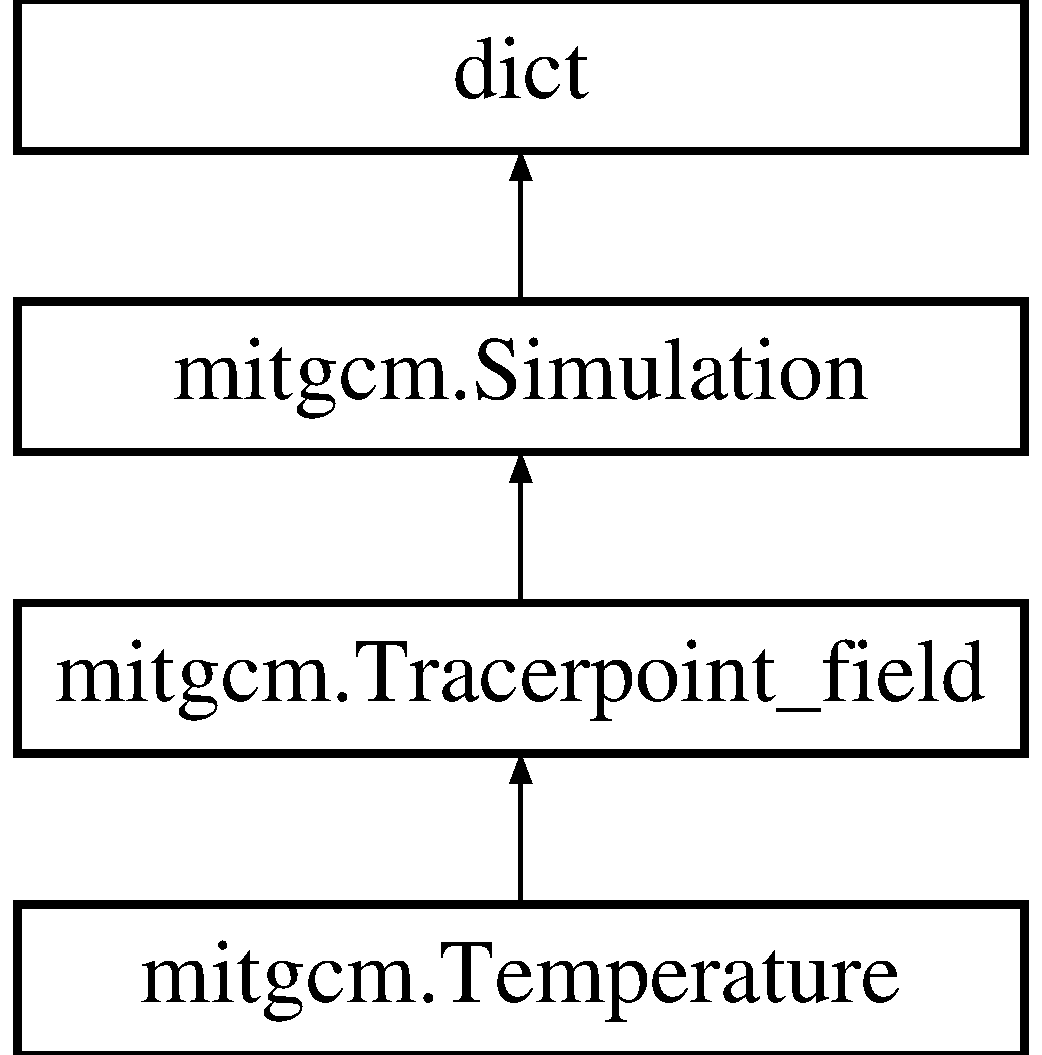
\includegraphics[height=4.000000cm]{classmitgcm_1_1Temperature}
\end{center}
\end{figure}
\subsection*{Public Member Functions}
\begin{DoxyCompactItemize}
\item 
\hypertarget{classmitgcm_1_1Temperature_af8a4e75bd94a1c6ab81f96ef0c4179f7}{def {\bfseries \+\_\+\+\_\+init\+\_\+\+\_\+}}\label{classmitgcm_1_1Temperature_af8a4e75bd94a1c6ab81f96ef0c4179f7}

\end{DoxyCompactItemize}
\subsection*{Additional Inherited Members}


\subsection{Detailed Description}


Definition at line 630 of file \+\_\+\+\_\+init\+\_\+\+\_\+.\+py.



The documentation for this class was generated from the following file\+:\begin{DoxyCompactItemize}
\item 
\+\_\+\+\_\+init\+\_\+\+\_\+.\+py\end{DoxyCompactItemize}

\hypertarget{classmitgcm_1_1Tracerpoint__field}{\section{mitgcm.\+Tracerpoint\+\_\+field Class Reference}
\label{classmitgcm_1_1Tracerpoint__field}\index{mitgcm.\+Tracerpoint\+\_\+field@{mitgcm.\+Tracerpoint\+\_\+field}}
}


This is the base class for all model fields on the tracer points.  


Inheritance diagram for mitgcm.\+Tracerpoint\+\_\+field\+:\begin{figure}[H]
\begin{center}
\leavevmode
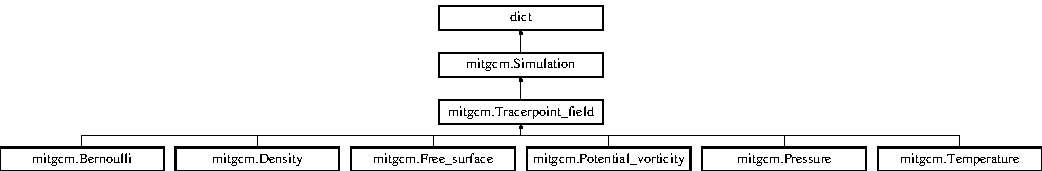
\includegraphics[height=2.304527cm]{classmitgcm_1_1Tracerpoint__field}
\end{center}
\end{figure}
\subsection*{Public Member Functions}
\begin{DoxyCompactItemize}
\item 
def \hyperlink{classmitgcm_1_1Tracerpoint__field_aaf8a54b25699658f016209c2624ccaac}{take\+\_\+d\+\_\+dx}
\begin{DoxyCompactList}\small\item\em Take the x derivative of the field on tracer points, using spacings in grid object. \end{DoxyCompactList}\item 
def \hyperlink{classmitgcm_1_1Tracerpoint__field_abe875d49041c764c65b579c6a0ba6c13}{take\+\_\+d\+\_\+dy}
\begin{DoxyCompactList}\small\item\em Take the y derivative of the field on tracer points, using spacings in grid object. \end{DoxyCompactList}\item 
def \hyperlink{classmitgcm_1_1Tracerpoint__field_aae9d224b41b5cf62433fd5fe473a8116}{take\+\_\+d\+\_\+dz}
\begin{DoxyCompactList}\small\item\em Take the z derivative of the field given on tracer-\/points, using the spacings in grid object. \end{DoxyCompactList}\end{DoxyCompactItemize}
\subsection*{Additional Inherited Members}


\subsection{Detailed Description}
This is the base class for all model fields on the tracer points. 

It includes definitions for taking derivatives. 

Definition at line 425 of file \+\_\+\+\_\+init\+\_\+\+\_\+.\+py.



\subsection{Member Function Documentation}
\hypertarget{classmitgcm_1_1Tracerpoint__field_aaf8a54b25699658f016209c2624ccaac}{\index{mitgcm\+::\+Tracerpoint\+\_\+field@{mitgcm\+::\+Tracerpoint\+\_\+field}!take\+\_\+d\+\_\+dx@{take\+\_\+d\+\_\+dx}}
\index{take\+\_\+d\+\_\+dx@{take\+\_\+d\+\_\+dx}!mitgcm\+::\+Tracerpoint\+\_\+field@{mitgcm\+::\+Tracerpoint\+\_\+field}}
\subsubsection[{take\+\_\+d\+\_\+dx}]{\setlength{\rightskip}{0pt plus 5cm}def mitgcm.\+Tracerpoint\+\_\+field.\+take\+\_\+d\+\_\+dx (
\begin{DoxyParamCaption}
\item[{}]{self, }
\item[{}]{model\+\_\+instance, }
\item[{}]{input\+\_\+field = {\ttfamily 'RHO'}, }
\item[{}]{output\+\_\+field = {\ttfamily 'dRHO\+\_\+dx'}}
\end{DoxyParamCaption}
)}}\label{classmitgcm_1_1Tracerpoint__field_aaf8a54b25699658f016209c2624ccaac}


Take the x derivative of the field on tracer points, using spacings in grid object. 

Performs centred second-\/order differencing everywhere except next to boundaries. First order is used there (meaning the gradients at the boundary are evaluated half a grid point away from where they should be). 

Definition at line 433 of file \+\_\+\+\_\+init\+\_\+\+\_\+.\+py.

\hypertarget{classmitgcm_1_1Tracerpoint__field_abe875d49041c764c65b579c6a0ba6c13}{\index{mitgcm\+::\+Tracerpoint\+\_\+field@{mitgcm\+::\+Tracerpoint\+\_\+field}!take\+\_\+d\+\_\+dy@{take\+\_\+d\+\_\+dy}}
\index{take\+\_\+d\+\_\+dy@{take\+\_\+d\+\_\+dy}!mitgcm\+::\+Tracerpoint\+\_\+field@{mitgcm\+::\+Tracerpoint\+\_\+field}}
\subsubsection[{take\+\_\+d\+\_\+dy}]{\setlength{\rightskip}{0pt plus 5cm}def mitgcm.\+Tracerpoint\+\_\+field.\+take\+\_\+d\+\_\+dy (
\begin{DoxyParamCaption}
\item[{}]{self, }
\item[{}]{model\+\_\+instance, }
\item[{}]{input\+\_\+field = {\ttfamily 'RHO'}, }
\item[{}]{output\+\_\+field = {\ttfamily 'dRHO\+\_\+dy'}}
\end{DoxyParamCaption}
)}}\label{classmitgcm_1_1Tracerpoint__field_abe875d49041c764c65b579c6a0ba6c13}


Take the y derivative of the field on tracer points, using spacings in grid object. 

Performs centred second-\/order differencing everywhere except next to boundaries. First order is used there (meaning the gradients at the boundary are evaluated half a grid point away from where they should be). 

Definition at line 464 of file \+\_\+\+\_\+init\+\_\+\+\_\+.\+py.

\hypertarget{classmitgcm_1_1Tracerpoint__field_aae9d224b41b5cf62433fd5fe473a8116}{\index{mitgcm\+::\+Tracerpoint\+\_\+field@{mitgcm\+::\+Tracerpoint\+\_\+field}!take\+\_\+d\+\_\+dz@{take\+\_\+d\+\_\+dz}}
\index{take\+\_\+d\+\_\+dz@{take\+\_\+d\+\_\+dz}!mitgcm\+::\+Tracerpoint\+\_\+field@{mitgcm\+::\+Tracerpoint\+\_\+field}}
\subsubsection[{take\+\_\+d\+\_\+dz}]{\setlength{\rightskip}{0pt plus 5cm}def mitgcm.\+Tracerpoint\+\_\+field.\+take\+\_\+d\+\_\+dz (
\begin{DoxyParamCaption}
\item[{}]{self, }
\item[{}]{model\+\_\+instance, }
\item[{}]{input\+\_\+field = {\ttfamily 'RHO'}, }
\item[{}]{output\+\_\+field = {\ttfamily 'dRHO\+\_\+dz'}}
\end{DoxyParamCaption}
)}}\label{classmitgcm_1_1Tracerpoint__field_aae9d224b41b5cf62433fd5fe473a8116}


Take the z derivative of the field given on tracer-\/points, using the spacings in grid object. 

Performs centred second-\/order differencing everywhere except next to boundaries. First order is used there (meaning the gradients at the boundary are evaluated half a grid point away from where they should be). 

Definition at line 495 of file \+\_\+\+\_\+init\+\_\+\+\_\+.\+py.



The documentation for this class was generated from the following file\+:\begin{DoxyCompactItemize}
\item 
\+\_\+\+\_\+init\+\_\+\+\_\+.\+py\end{DoxyCompactItemize}

\hypertarget{classmitgcm_1_1Upoint__field}{}\section{mitgcm.\+Upoint\+\_\+field Class Reference}
\label{classmitgcm_1_1Upoint__field}\index{mitgcm.\+Upoint\+\_\+field@{mitgcm.\+Upoint\+\_\+field}}
Inheritance diagram for mitgcm.\+Upoint\+\_\+field\+:\begin{figure}[H]
\begin{center}
\leavevmode
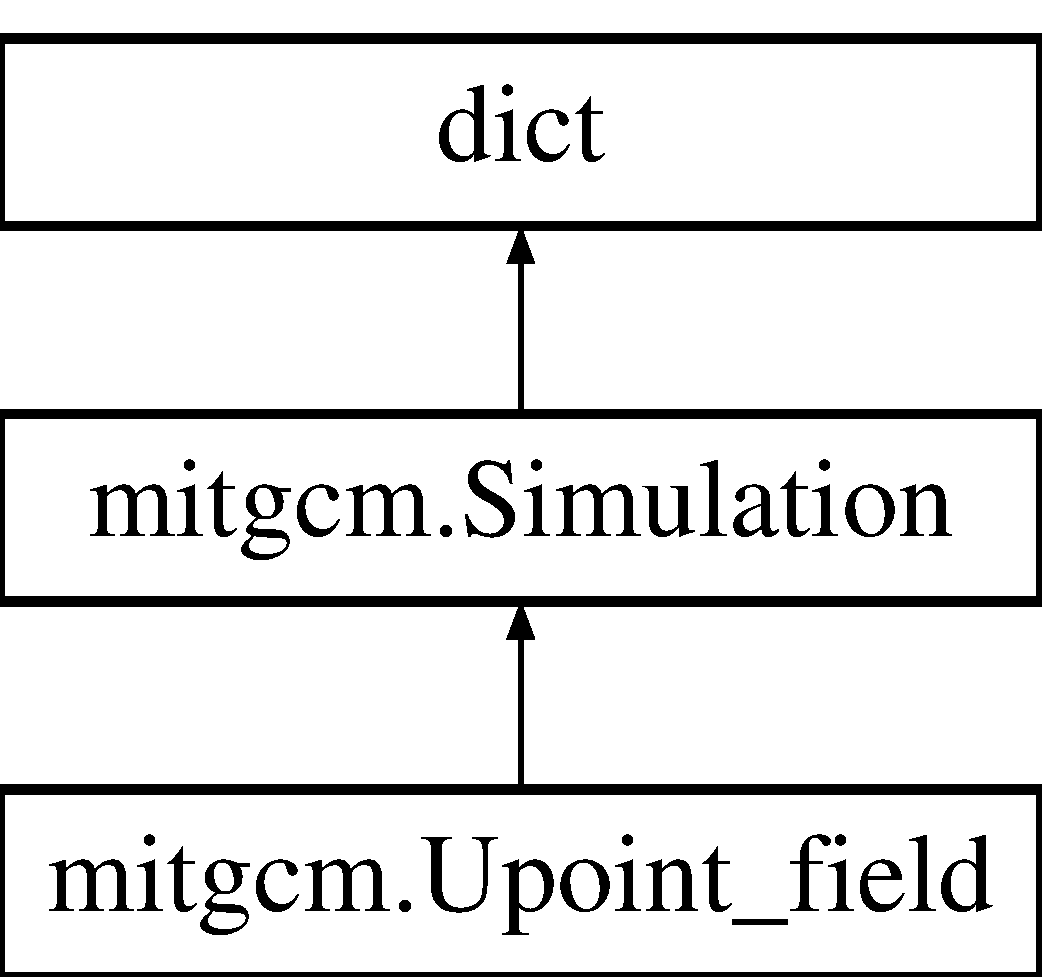
\includegraphics[height=3.000000cm]{classmitgcm_1_1Upoint__field}
\end{center}
\end{figure}
\subsection*{Public Member Functions}
\begin{DoxyCompactItemize}
\item 
\hypertarget{classmitgcm_1_1Upoint__field_a4b4f700e8387298d0a1373285594d0fb}{}def {\bfseries \+\_\+\+\_\+init\+\_\+\+\_\+} (self, netcdf\+\_\+filename, variable, time\+\_\+level)\label{classmitgcm_1_1Upoint__field_a4b4f700e8387298d0a1373285594d0fb}

\item 
def \hyperlink{classmitgcm_1_1Upoint__field_a3f136fd99e5a7ce04aef0f216bd32019}{take\+\_\+d\+\_\+dx}
\begin{DoxyCompactList}\small\item\em Derivatives of model fields. \end{DoxyCompactList}\item 
def \hyperlink{classmitgcm_1_1Upoint__field_acf9bf315e3d31834781c0642086a7802}{take\+\_\+d\+\_\+dy}
\begin{DoxyCompactList}\small\item\em Take the y derivative of the field on u points, using the spacings provided. \end{DoxyCompactList}\item 
def \hyperlink{classmitgcm_1_1Upoint__field_a8bfdba5354910eed3e9e8827d38608f8}{take\+\_\+d\+\_\+dz}
\begin{DoxyCompactList}\small\item\em Take the z derivative of the field given on u-\/points, using the spacings in grid object. \end{DoxyCompactList}\end{DoxyCompactItemize}
\subsection*{Additional Inherited Members}


\subsection{Detailed Description}


Definition at line 89 of file \+\_\+\+\_\+init\+\_\+\+\_\+.\+py.



\subsection{Member Function Documentation}
\hypertarget{classmitgcm_1_1Upoint__field_a3f136fd99e5a7ce04aef0f216bd32019}{}\index{mitgcm\+::\+Upoint\+\_\+field@{mitgcm\+::\+Upoint\+\_\+field}!take\+\_\+d\+\_\+dx@{take\+\_\+d\+\_\+dx}}
\index{take\+\_\+d\+\_\+dx@{take\+\_\+d\+\_\+dx}!mitgcm\+::\+Upoint\+\_\+field@{mitgcm\+::\+Upoint\+\_\+field}}
\subsubsection[{take\+\_\+d\+\_\+dx}]{\setlength{\rightskip}{0pt plus 5cm}def mitgcm.\+Upoint\+\_\+field.\+take\+\_\+d\+\_\+dx (
\begin{DoxyParamCaption}
\item[{}]{self, }
\item[{}]{model\+\_\+instance, }
\item[{}]{input\+\_\+field = {\ttfamily \textquotesingle{}UVEL\textquotesingle{}}, }
\item[{}]{output\+\_\+field = {\ttfamily \textquotesingle{}dU\+\_\+dx\textquotesingle{}}}
\end{DoxyParamCaption}
)}\label{classmitgcm_1_1Upoint__field_a3f136fd99e5a7ce04aef0f216bd32019}


Derivatives of model fields. 

Take the x derivative of the field given on u-\/points, using the spacings in grid object. \begin{DoxyVerb}   Performs centred second-order differencing everywhere except next to boundaries. First order is 
   used there (meaning the gradients at the boundary are evaluated half a grid point away from where 
   they should be). \end{DoxyVerb}
 

Definition at line 106 of file \+\_\+\+\_\+init\+\_\+\+\_\+.\+py.

\hypertarget{classmitgcm_1_1Upoint__field_acf9bf315e3d31834781c0642086a7802}{}\index{mitgcm\+::\+Upoint\+\_\+field@{mitgcm\+::\+Upoint\+\_\+field}!take\+\_\+d\+\_\+dy@{take\+\_\+d\+\_\+dy}}
\index{take\+\_\+d\+\_\+dy@{take\+\_\+d\+\_\+dy}!mitgcm\+::\+Upoint\+\_\+field@{mitgcm\+::\+Upoint\+\_\+field}}
\subsubsection[{take\+\_\+d\+\_\+dy}]{\setlength{\rightskip}{0pt plus 5cm}def mitgcm.\+Upoint\+\_\+field.\+take\+\_\+d\+\_\+dy (
\begin{DoxyParamCaption}
\item[{}]{self, }
\item[{}]{model\+\_\+instance, }
\item[{}]{input\+\_\+field = {\ttfamily \textquotesingle{}UVEL\textquotesingle{}}, }
\item[{}]{output\+\_\+field = {\ttfamily \textquotesingle{}dU\+\_\+dy\textquotesingle{}}}
\end{DoxyParamCaption}
)}\label{classmitgcm_1_1Upoint__field_acf9bf315e3d31834781c0642086a7802}


Take the y derivative of the field on u points, using the spacings provided. 

Performs centred second-\/order differencing everywhere except next to boundaries. First order is used there (meaning the gradients at the boundary are evaluated half a grid point away from where they should be). 

Definition at line 141 of file \+\_\+\+\_\+init\+\_\+\+\_\+.\+py.

\hypertarget{classmitgcm_1_1Upoint__field_a8bfdba5354910eed3e9e8827d38608f8}{}\index{mitgcm\+::\+Upoint\+\_\+field@{mitgcm\+::\+Upoint\+\_\+field}!take\+\_\+d\+\_\+dz@{take\+\_\+d\+\_\+dz}}
\index{take\+\_\+d\+\_\+dz@{take\+\_\+d\+\_\+dz}!mitgcm\+::\+Upoint\+\_\+field@{mitgcm\+::\+Upoint\+\_\+field}}
\subsubsection[{take\+\_\+d\+\_\+dz}]{\setlength{\rightskip}{0pt plus 5cm}def mitgcm.\+Upoint\+\_\+field.\+take\+\_\+d\+\_\+dz (
\begin{DoxyParamCaption}
\item[{}]{self, }
\item[{}]{model\+\_\+instance, }
\item[{}]{input\+\_\+field = {\ttfamily \textquotesingle{}UVEL\textquotesingle{}}, }
\item[{}]{output\+\_\+field = {\ttfamily \textquotesingle{}dU\+\_\+dz\textquotesingle{}}}
\end{DoxyParamCaption}
)}\label{classmitgcm_1_1Upoint__field_a8bfdba5354910eed3e9e8827d38608f8}


Take the z derivative of the field given on u-\/points, using the spacings in grid object. 

Performs centred second-\/order differencing everywhere except next to boundaries. First order is used there (meaning the gradients at the boundary are evaluated half a grid point away from where they should be). 

Definition at line 177 of file \+\_\+\+\_\+init\+\_\+\+\_\+.\+py.



The documentation for this class was generated from the following file\+:\begin{DoxyCompactItemize}
\item 
\+\_\+\+\_\+init\+\_\+\+\_\+.\+py\end{DoxyCompactItemize}

\hypertarget{classmitgcm_1_1Vorticity}{\section{mitgcm.\+Vorticity Class Reference}
\label{classmitgcm_1_1Vorticity}\index{mitgcm.\+Vorticity@{mitgcm.\+Vorticity}}
}
Inheritance diagram for mitgcm.\+Vorticity\+:\begin{figure}[H]
\begin{center}
\leavevmode
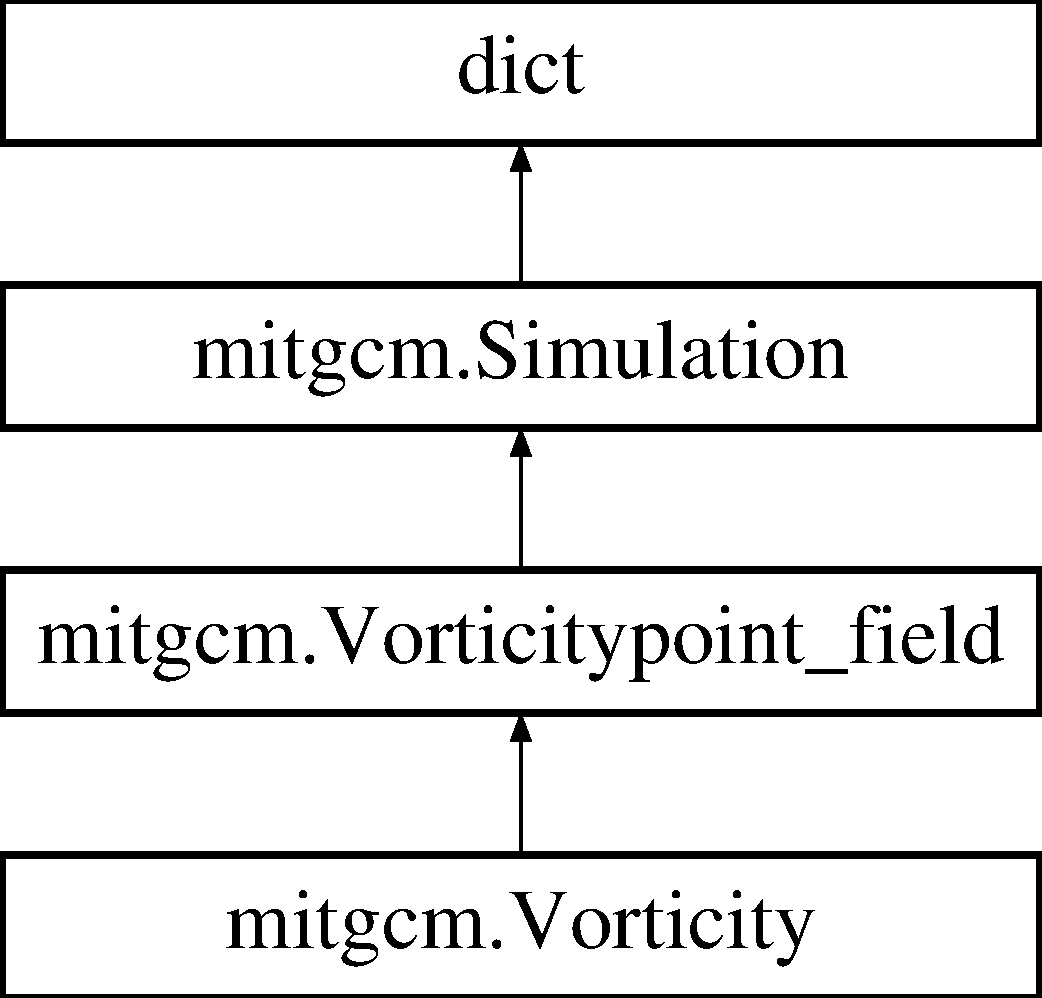
\includegraphics[height=4.000000cm]{classmitgcm_1_1Vorticity}
\end{center}
\end{figure}
\subsection*{Public Member Functions}
\begin{DoxyCompactItemize}
\item 
\hypertarget{classmitgcm_1_1Vorticity_a6fdcf74ea42dc79b3b8eab1eb2a149e4}{def {\bfseries \+\_\+\+\_\+init\+\_\+\+\_\+}}\label{classmitgcm_1_1Vorticity_a6fdcf74ea42dc79b3b8eab1eb2a149e4}

\end{DoxyCompactItemize}
\subsection*{Additional Inherited Members}


\subsection{Detailed Description}


Definition at line 710 of file \+\_\+\+\_\+init\+\_\+\+\_\+.\+py.



The documentation for this class was generated from the following file\+:\begin{DoxyCompactItemize}
\item 
\+\_\+\+\_\+init\+\_\+\+\_\+.\+py\end{DoxyCompactItemize}

\hypertarget{classmitgcm_1_1Vorticitypoint__field}{}\section{mitgcm.\+Vorticitypoint\+\_\+field Class Reference}
\label{classmitgcm_1_1Vorticitypoint__field}\index{mitgcm.\+Vorticitypoint\+\_\+field@{mitgcm.\+Vorticitypoint\+\_\+field}}
Inheritance diagram for mitgcm.\+Vorticitypoint\+\_\+field\+:\begin{figure}[H]
\begin{center}
\leavevmode
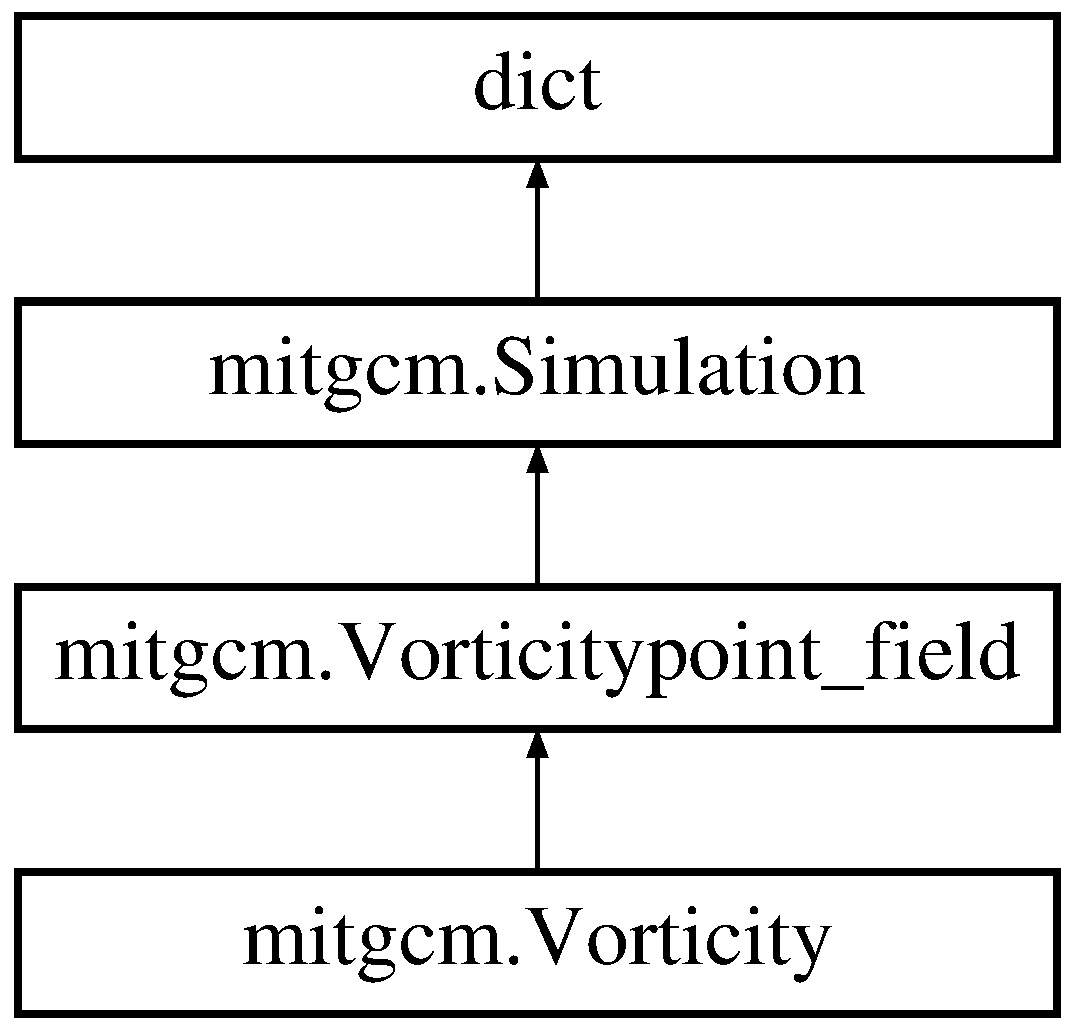
\includegraphics[height=4.000000cm]{classmitgcm_1_1Vorticitypoint__field}
\end{center}
\end{figure}
\subsection*{Additional Inherited Members}


\subsection{Detailed Description}


Definition at line 520 of file \+\_\+\+\_\+init\+\_\+\+\_\+.\+py.



The documentation for this class was generated from the following file\+:\begin{DoxyCompactItemize}
\item 
\+\_\+\+\_\+init\+\_\+\+\_\+.\+py\end{DoxyCompactItemize}

\hypertarget{classmitgcm_1_1Vpoint__field}{\section{mitgcm.\+Vpoint\+\_\+field Class Reference}
\label{classmitgcm_1_1Vpoint__field}\index{mitgcm.\+Vpoint\+\_\+field@{mitgcm.\+Vpoint\+\_\+field}}
}


This is the class fo rall fields on meridional velocity points.  


Inheritance diagram for mitgcm.\+Vpoint\+\_\+field\+:\begin{figure}[H]
\begin{center}
\leavevmode
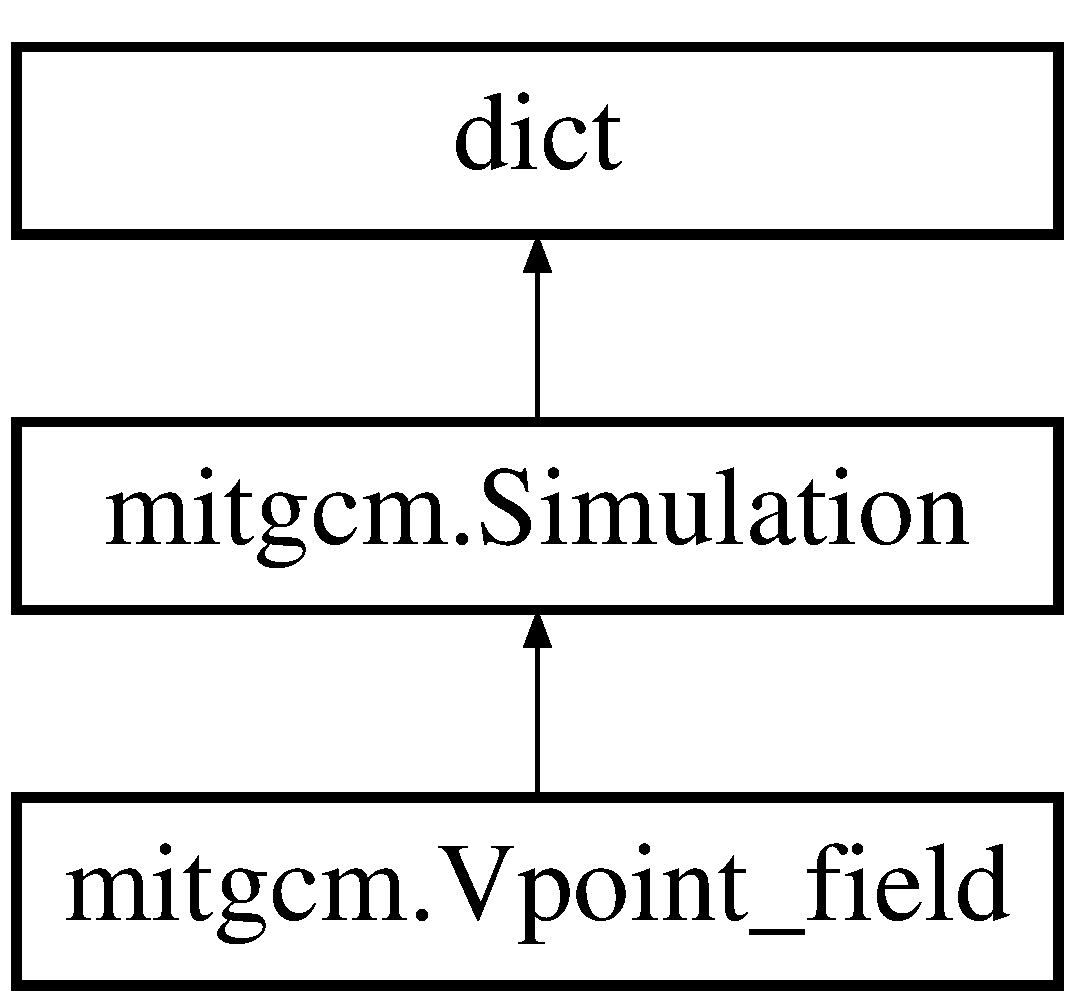
\includegraphics[height=3.000000cm]{classmitgcm_1_1Vpoint__field}
\end{center}
\end{figure}
\subsection*{Public Member Functions}
\begin{DoxyCompactItemize}
\item 
def \hyperlink{classmitgcm_1_1Vpoint__field_a0dead38b0594e3f722eec29586d0451a}{\+\_\+\+\_\+init\+\_\+\+\_\+}
\begin{DoxyCompactList}\small\item\em Instantiate a field on the meridional velocity points. \end{DoxyCompactList}\item 
def \hyperlink{classmitgcm_1_1Vpoint__field_a0735efcbc90505f47a507f102061f18a}{take\+\_\+d\+\_\+dx}
\begin{DoxyCompactList}\small\item\em Take the x derivative of the field on v points using the spacings in model\+\_\+instance.\+grid object. \end{DoxyCompactList}\item 
def \hyperlink{classmitgcm_1_1Vpoint__field_acaccb1a41ec42c0f60c82bf092534b94}{take\+\_\+d\+\_\+dy}
\begin{DoxyCompactList}\small\item\em Take the y derivative of the field given on v-\/points, using the spacings in grid object. \end{DoxyCompactList}\item 
def \hyperlink{classmitgcm_1_1Vpoint__field_a6d06f4b2a5e774bbc711e39ba51723ea}{take\+\_\+d\+\_\+dz}
\begin{DoxyCompactList}\small\item\em Take the z derivative of the field given on v-\/points, using the spacings in grid object. \end{DoxyCompactList}\end{DoxyCompactItemize}
\subsection*{Additional Inherited Members}


\subsection{Detailed Description}
This is the class fo rall fields on meridional velocity points. 



Definition at line 206 of file \+\_\+\+\_\+init\+\_\+\+\_\+.\+py.



\subsection{Constructor \& Destructor Documentation}
\hypertarget{classmitgcm_1_1Vpoint__field_a0dead38b0594e3f722eec29586d0451a}{\index{mitgcm\+::\+Vpoint\+\_\+field@{mitgcm\+::\+Vpoint\+\_\+field}!\+\_\+\+\_\+init\+\_\+\+\_\+@{\+\_\+\+\_\+init\+\_\+\+\_\+}}
\index{\+\_\+\+\_\+init\+\_\+\+\_\+@{\+\_\+\+\_\+init\+\_\+\+\_\+}!mitgcm\+::\+Vpoint\+\_\+field@{mitgcm\+::\+Vpoint\+\_\+field}}
\subsubsection[{\+\_\+\+\_\+init\+\_\+\+\_\+}]{\setlength{\rightskip}{0pt plus 5cm}def mitgcm.\+Vpoint\+\_\+field.\+\_\+\+\_\+init\+\_\+\+\_\+ (
\begin{DoxyParamCaption}
\item[{}]{self, }
\item[{}]{netcdf\+\_\+filename, }
\item[{}]{variable, }
\item[{}]{time\+\_\+level}
\end{DoxyParamCaption}
)}}\label{classmitgcm_1_1Vpoint__field_a0dead38b0594e3f722eec29586d0451a}


Instantiate a field on the meridional velocity points. 



Definition at line 210 of file \+\_\+\+\_\+init\+\_\+\+\_\+.\+py.



\subsection{Member Function Documentation}
\hypertarget{classmitgcm_1_1Vpoint__field_a0735efcbc90505f47a507f102061f18a}{\index{mitgcm\+::\+Vpoint\+\_\+field@{mitgcm\+::\+Vpoint\+\_\+field}!take\+\_\+d\+\_\+dx@{take\+\_\+d\+\_\+dx}}
\index{take\+\_\+d\+\_\+dx@{take\+\_\+d\+\_\+dx}!mitgcm\+::\+Vpoint\+\_\+field@{mitgcm\+::\+Vpoint\+\_\+field}}
\subsubsection[{take\+\_\+d\+\_\+dx}]{\setlength{\rightskip}{0pt plus 5cm}def mitgcm.\+Vpoint\+\_\+field.\+take\+\_\+d\+\_\+dx (
\begin{DoxyParamCaption}
\item[{}]{self, }
\item[{}]{model\+\_\+instance, }
\item[{}]{input\+\_\+field = {\ttfamily 'VVEL'}, }
\item[{}]{output\+\_\+field = {\ttfamily 'dV\+\_\+dx'}}
\end{DoxyParamCaption}
)}}\label{classmitgcm_1_1Vpoint__field_a0735efcbc90505f47a507f102061f18a}


Take the x derivative of the field on v points using the spacings in model\+\_\+instance.\+grid object. 

This function can be daisy-\/chained to get higher order derivatives.

Performs centred second-\/order differencing everywhere except next to boundaries. First order is used there (meaning the gradients at the boundary are evaluated half a grid point away from where they should be). 

Definition at line 227 of file \+\_\+\+\_\+init\+\_\+\+\_\+.\+py.

\hypertarget{classmitgcm_1_1Vpoint__field_acaccb1a41ec42c0f60c82bf092534b94}{\index{mitgcm\+::\+Vpoint\+\_\+field@{mitgcm\+::\+Vpoint\+\_\+field}!take\+\_\+d\+\_\+dy@{take\+\_\+d\+\_\+dy}}
\index{take\+\_\+d\+\_\+dy@{take\+\_\+d\+\_\+dy}!mitgcm\+::\+Vpoint\+\_\+field@{mitgcm\+::\+Vpoint\+\_\+field}}
\subsubsection[{take\+\_\+d\+\_\+dy}]{\setlength{\rightskip}{0pt plus 5cm}def mitgcm.\+Vpoint\+\_\+field.\+take\+\_\+d\+\_\+dy (
\begin{DoxyParamCaption}
\item[{}]{self, }
\item[{}]{model\+\_\+instance, }
\item[{}]{input\+\_\+field = {\ttfamily 'VVEL'}, }
\item[{}]{output\+\_\+field = {\ttfamily 'dV\+\_\+dy'}}
\end{DoxyParamCaption}
)}}\label{classmitgcm_1_1Vpoint__field_acaccb1a41ec42c0f60c82bf092534b94}


Take the y derivative of the field given on v-\/points, using the spacings in grid object. 

Performs centred second-\/order differencing everywhere except next to boundaries. First order is used there (meaning the gradients at the boundary are evaluated half a grid point away from where they should be). 

Definition at line 258 of file \+\_\+\+\_\+init\+\_\+\+\_\+.\+py.

\hypertarget{classmitgcm_1_1Vpoint__field_a6d06f4b2a5e774bbc711e39ba51723ea}{\index{mitgcm\+::\+Vpoint\+\_\+field@{mitgcm\+::\+Vpoint\+\_\+field}!take\+\_\+d\+\_\+dz@{take\+\_\+d\+\_\+dz}}
\index{take\+\_\+d\+\_\+dz@{take\+\_\+d\+\_\+dz}!mitgcm\+::\+Vpoint\+\_\+field@{mitgcm\+::\+Vpoint\+\_\+field}}
\subsubsection[{take\+\_\+d\+\_\+dz}]{\setlength{\rightskip}{0pt plus 5cm}def mitgcm.\+Vpoint\+\_\+field.\+take\+\_\+d\+\_\+dz (
\begin{DoxyParamCaption}
\item[{}]{self, }
\item[{}]{model\+\_\+instance, }
\item[{}]{input\+\_\+field = {\ttfamily 'VVEL'}, }
\item[{}]{output\+\_\+field = {\ttfamily 'dV\+\_\+dz'}}
\end{DoxyParamCaption}
)}}\label{classmitgcm_1_1Vpoint__field_a6d06f4b2a5e774bbc711e39ba51723ea}


Take the z derivative of the field given on v-\/points, using the spacings in grid object. 

Performs centred second-\/order differencing everywhere except next to boundaries. First order is used there (meaning the gradients at the boundary are evaluated half a grid point away from where they should be). 

Definition at line 290 of file \+\_\+\+\_\+init\+\_\+\+\_\+.\+py.



The documentation for this class was generated from the following file\+:\begin{DoxyCompactItemize}
\item 
\+\_\+\+\_\+init\+\_\+\+\_\+.\+py\end{DoxyCompactItemize}

\hypertarget{classmitgcm_1_1Wpoint__field}{}\section{mitgcm.\+Wpoint\+\_\+field Class Reference}
\label{classmitgcm_1_1Wpoint__field}\index{mitgcm.\+Wpoint\+\_\+field@{mitgcm.\+Wpoint\+\_\+field}}
Inheritance diagram for mitgcm.\+Wpoint\+\_\+field\+:\begin{figure}[H]
\begin{center}
\leavevmode
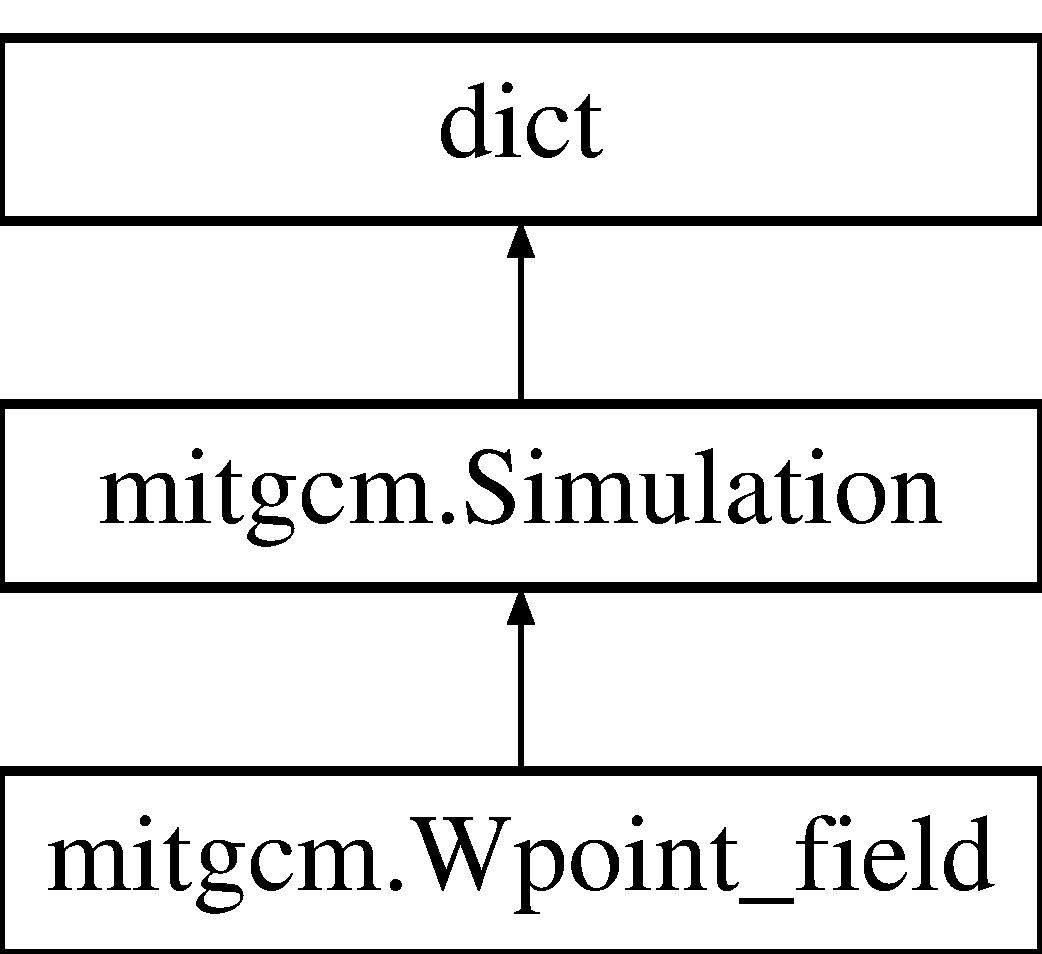
\includegraphics[height=3.000000cm]{classmitgcm_1_1Wpoint__field}
\end{center}
\end{figure}
\subsection*{Public Member Functions}
\begin{DoxyCompactItemize}
\item 
\hypertarget{classmitgcm_1_1Wpoint__field_a2a5c51740d3b21316f8a47e14ff948bf}{}def {\bfseries \+\_\+\+\_\+init\+\_\+\+\_\+} (self, netcdf\+\_\+filename, variable, time\+\_\+level)\label{classmitgcm_1_1Wpoint__field_a2a5c51740d3b21316f8a47e14ff948bf}

\item 
def \hyperlink{classmitgcm_1_1Wpoint__field_a9d36e2a9cc0545fb08a7b914968aa75a}{take\+\_\+d\+\_\+dx}
\begin{DoxyCompactList}\small\item\em Take the x derivative of the field on w points, using spacings in grid object. \end{DoxyCompactList}\item 
def \hyperlink{classmitgcm_1_1Wpoint__field_a669146364af5537c435957e297b41f57}{take\+\_\+d\+\_\+dy}
\begin{DoxyCompactList}\small\item\em Take the y derivative of the field on w points, using spacings in grid object. \end{DoxyCompactList}\item 
def \hyperlink{classmitgcm_1_1Wpoint__field_a7edd07d71d411e7f41acb496cc054bd0}{take\+\_\+d\+\_\+dz}
\begin{DoxyCompactList}\small\item\em Take the z derivative of the field given on w-\/points, using the spacings in grid object. \end{DoxyCompactList}\end{DoxyCompactItemize}
\subsection*{Additional Inherited Members}


\subsection{Detailed Description}


Definition at line 307 of file \+\_\+\+\_\+init\+\_\+\+\_\+.\+py.



\subsection{Member Function Documentation}
\hypertarget{classmitgcm_1_1Wpoint__field_a9d36e2a9cc0545fb08a7b914968aa75a}{}\index{mitgcm\+::\+Wpoint\+\_\+field@{mitgcm\+::\+Wpoint\+\_\+field}!take\+\_\+d\+\_\+dx@{take\+\_\+d\+\_\+dx}}
\index{take\+\_\+d\+\_\+dx@{take\+\_\+d\+\_\+dx}!mitgcm\+::\+Wpoint\+\_\+field@{mitgcm\+::\+Wpoint\+\_\+field}}
\subsubsection[{take\+\_\+d\+\_\+dx}]{\setlength{\rightskip}{0pt plus 5cm}def mitgcm.\+Wpoint\+\_\+field.\+take\+\_\+d\+\_\+dx (
\begin{DoxyParamCaption}
\item[{}]{self, }
\item[{}]{model\+\_\+instance, }
\item[{}]{input\+\_\+field = {\ttfamily \textquotesingle{}WVEL\textquotesingle{}}, }
\item[{}]{output\+\_\+field = {\ttfamily \textquotesingle{}dW\+\_\+dx\textquotesingle{}}}
\end{DoxyParamCaption}
)}\label{classmitgcm_1_1Wpoint__field_a9d36e2a9cc0545fb08a7b914968aa75a}


Take the x derivative of the field on w points, using spacings in grid object. 

Performs centred second-\/order differencing everywhere except next to boundaries. First order is used there (meaning the gradients at the boundary are evaluated half a grid point away from where they should be). 

Definition at line 332 of file \+\_\+\+\_\+init\+\_\+\+\_\+.\+py.

\hypertarget{classmitgcm_1_1Wpoint__field_a669146364af5537c435957e297b41f57}{}\index{mitgcm\+::\+Wpoint\+\_\+field@{mitgcm\+::\+Wpoint\+\_\+field}!take\+\_\+d\+\_\+dy@{take\+\_\+d\+\_\+dy}}
\index{take\+\_\+d\+\_\+dy@{take\+\_\+d\+\_\+dy}!mitgcm\+::\+Wpoint\+\_\+field@{mitgcm\+::\+Wpoint\+\_\+field}}
\subsubsection[{take\+\_\+d\+\_\+dy}]{\setlength{\rightskip}{0pt plus 5cm}def mitgcm.\+Wpoint\+\_\+field.\+take\+\_\+d\+\_\+dy (
\begin{DoxyParamCaption}
\item[{}]{self, }
\item[{}]{model\+\_\+instance, }
\item[{}]{input\+\_\+field = {\ttfamily \textquotesingle{}WVEL\textquotesingle{}}, }
\item[{}]{output\+\_\+field = {\ttfamily \textquotesingle{}dW\+\_\+dy\textquotesingle{}}}
\end{DoxyParamCaption}
)}\label{classmitgcm_1_1Wpoint__field_a669146364af5537c435957e297b41f57}


Take the y derivative of the field on w points, using spacings in grid object. 

Performs centred second-\/order differencing everywhere except next to boundaries. First order is used there (meaning the gradients at the boundary are evaluated half a grid point away from where they should be). 

Definition at line 364 of file \+\_\+\+\_\+init\+\_\+\+\_\+.\+py.

\hypertarget{classmitgcm_1_1Wpoint__field_a7edd07d71d411e7f41acb496cc054bd0}{}\index{mitgcm\+::\+Wpoint\+\_\+field@{mitgcm\+::\+Wpoint\+\_\+field}!take\+\_\+d\+\_\+dz@{take\+\_\+d\+\_\+dz}}
\index{take\+\_\+d\+\_\+dz@{take\+\_\+d\+\_\+dz}!mitgcm\+::\+Wpoint\+\_\+field@{mitgcm\+::\+Wpoint\+\_\+field}}
\subsubsection[{take\+\_\+d\+\_\+dz}]{\setlength{\rightskip}{0pt plus 5cm}def mitgcm.\+Wpoint\+\_\+field.\+take\+\_\+d\+\_\+dz (
\begin{DoxyParamCaption}
\item[{}]{self, }
\item[{}]{model\+\_\+instance, }
\item[{}]{input\+\_\+field = {\ttfamily \textquotesingle{}WVEL\textquotesingle{}}, }
\item[{}]{output\+\_\+field = {\ttfamily \textquotesingle{}dW\+\_\+dz\textquotesingle{}}}
\end{DoxyParamCaption}
)}\label{classmitgcm_1_1Wpoint__field_a7edd07d71d411e7f41acb496cc054bd0}


Take the z derivative of the field given on w-\/points, using the spacings in grid object. 

Performs centred second-\/order differencing everywhere except next to boundaries. First order is used there (meaning the gradients at the boundary are evaluated half a grid point away from where they should be). 

Definition at line 395 of file \+\_\+\+\_\+init\+\_\+\+\_\+.\+py.



The documentation for this class was generated from the following file\+:\begin{DoxyCompactItemize}
\item 
\+\_\+\+\_\+init\+\_\+\+\_\+.\+py\end{DoxyCompactItemize}

%--- End generated contents ---

% Index
\newpage
\phantomsection
\addcontentsline{toc}{chapter}{Index}
\printindex

\end{document}
